% Options for packages loaded elsewhere
\PassOptionsToPackage{unicode}{hyperref}
\PassOptionsToPackage{hyphens}{url}
%
\documentclass[
]{book}
\usepackage{lmodern}
\usepackage{amssymb,amsmath}
\usepackage{ifxetex,ifluatex}
\ifnum 0\ifxetex 1\fi\ifluatex 1\fi=0 % if pdftex
  \usepackage[T1]{fontenc}
  \usepackage[utf8]{inputenc}
  \usepackage{textcomp} % provide euro and other symbols
\else % if luatex or xetex
  \usepackage{unicode-math}
  \defaultfontfeatures{Scale=MatchLowercase}
  \defaultfontfeatures[\rmfamily]{Ligatures=TeX,Scale=1}
\fi
% Use upquote if available, for straight quotes in verbatim environments
\IfFileExists{upquote.sty}{\usepackage{upquote}}{}
\IfFileExists{microtype.sty}{% use microtype if available
  \usepackage[]{microtype}
  \UseMicrotypeSet[protrusion]{basicmath} % disable protrusion for tt fonts
}{}
\makeatletter
\@ifundefined{KOMAClassName}{% if non-KOMA class
  \IfFileExists{parskip.sty}{%
    \usepackage{parskip}
  }{% else
    \setlength{\parindent}{0pt}
    \setlength{\parskip}{6pt plus 2pt minus 1pt}}
}{% if KOMA class
  \KOMAoptions{parskip=half}}
\makeatother
\usepackage{xcolor}
\IfFileExists{xurl.sty}{\usepackage{xurl}}{} % add URL line breaks if available
\IfFileExists{bookmark.sty}{\usepackage{bookmark}}{\usepackage{hyperref}}
\hypersetup{
  pdftitle={Laboratório de Sistemas de Controle},
  pdfauthor={Djonathan Luiz de Oliveira Quadras},
  hidelinks,
  pdfcreator={LaTeX via pandoc}}
\urlstyle{same} % disable monospaced font for URLs
\usepackage{color}
\usepackage{fancyvrb}
\newcommand{\VerbBar}{|}
\newcommand{\VERB}{\Verb[commandchars=\\\{\}]}
\DefineVerbatimEnvironment{Highlighting}{Verbatim}{commandchars=\\\{\}}
% Add ',fontsize=\small' for more characters per line
\usepackage{framed}
\definecolor{shadecolor}{RGB}{248,248,248}
\newenvironment{Shaded}{\begin{snugshade}}{\end{snugshade}}
\newcommand{\AlertTok}[1]{\textcolor[rgb]{0.94,0.16,0.16}{#1}}
\newcommand{\AnnotationTok}[1]{\textcolor[rgb]{0.56,0.35,0.01}{\textbf{\textit{#1}}}}
\newcommand{\AttributeTok}[1]{\textcolor[rgb]{0.77,0.63,0.00}{#1}}
\newcommand{\BaseNTok}[1]{\textcolor[rgb]{0.00,0.00,0.81}{#1}}
\newcommand{\BuiltInTok}[1]{#1}
\newcommand{\CharTok}[1]{\textcolor[rgb]{0.31,0.60,0.02}{#1}}
\newcommand{\CommentTok}[1]{\textcolor[rgb]{0.56,0.35,0.01}{\textit{#1}}}
\newcommand{\CommentVarTok}[1]{\textcolor[rgb]{0.56,0.35,0.01}{\textbf{\textit{#1}}}}
\newcommand{\ConstantTok}[1]{\textcolor[rgb]{0.00,0.00,0.00}{#1}}
\newcommand{\ControlFlowTok}[1]{\textcolor[rgb]{0.13,0.29,0.53}{\textbf{#1}}}
\newcommand{\DataTypeTok}[1]{\textcolor[rgb]{0.13,0.29,0.53}{#1}}
\newcommand{\DecValTok}[1]{\textcolor[rgb]{0.00,0.00,0.81}{#1}}
\newcommand{\DocumentationTok}[1]{\textcolor[rgb]{0.56,0.35,0.01}{\textbf{\textit{#1}}}}
\newcommand{\ErrorTok}[1]{\textcolor[rgb]{0.64,0.00,0.00}{\textbf{#1}}}
\newcommand{\ExtensionTok}[1]{#1}
\newcommand{\FloatTok}[1]{\textcolor[rgb]{0.00,0.00,0.81}{#1}}
\newcommand{\FunctionTok}[1]{\textcolor[rgb]{0.00,0.00,0.00}{#1}}
\newcommand{\ImportTok}[1]{#1}
\newcommand{\InformationTok}[1]{\textcolor[rgb]{0.56,0.35,0.01}{\textbf{\textit{#1}}}}
\newcommand{\KeywordTok}[1]{\textcolor[rgb]{0.13,0.29,0.53}{\textbf{#1}}}
\newcommand{\NormalTok}[1]{#1}
\newcommand{\OperatorTok}[1]{\textcolor[rgb]{0.81,0.36,0.00}{\textbf{#1}}}
\newcommand{\OtherTok}[1]{\textcolor[rgb]{0.56,0.35,0.01}{#1}}
\newcommand{\PreprocessorTok}[1]{\textcolor[rgb]{0.56,0.35,0.01}{\textit{#1}}}
\newcommand{\RegionMarkerTok}[1]{#1}
\newcommand{\SpecialCharTok}[1]{\textcolor[rgb]{0.00,0.00,0.00}{#1}}
\newcommand{\SpecialStringTok}[1]{\textcolor[rgb]{0.31,0.60,0.02}{#1}}
\newcommand{\StringTok}[1]{\textcolor[rgb]{0.31,0.60,0.02}{#1}}
\newcommand{\VariableTok}[1]{\textcolor[rgb]{0.00,0.00,0.00}{#1}}
\newcommand{\VerbatimStringTok}[1]{\textcolor[rgb]{0.31,0.60,0.02}{#1}}
\newcommand{\WarningTok}[1]{\textcolor[rgb]{0.56,0.35,0.01}{\textbf{\textit{#1}}}}
\usepackage{longtable,booktabs}
% Correct order of tables after \paragraph or \subparagraph
\usepackage{etoolbox}
\makeatletter
\patchcmd\longtable{\par}{\if@noskipsec\mbox{}\fi\par}{}{}
\makeatother
% Allow footnotes in longtable head/foot
\IfFileExists{footnotehyper.sty}{\usepackage{footnotehyper}}{\usepackage{footnote}}
\makesavenoteenv{longtable}
\usepackage{graphicx}
\makeatletter
\def\maxwidth{\ifdim\Gin@nat@width>\linewidth\linewidth\else\Gin@nat@width\fi}
\def\maxheight{\ifdim\Gin@nat@height>\textheight\textheight\else\Gin@nat@height\fi}
\makeatother
% Scale images if necessary, so that they will not overflow the page
% margins by default, and it is still possible to overwrite the defaults
% using explicit options in \includegraphics[width, height, ...]{}
\setkeys{Gin}{width=\maxwidth,height=\maxheight,keepaspectratio}
% Set default figure placement to htbp
\makeatletter
\def\fps@figure{htbp}
\makeatother
\setlength{\emergencystretch}{3em} % prevent overfull lines
\providecommand{\tightlist}{%
  \setlength{\itemsep}{0pt}\setlength{\parskip}{0pt}}
\setcounter{secnumdepth}{5}
\usepackage{booktabs}
\usepackage[]{natbib}
\bibliographystyle{apalike}

\title{Laboratório de Sistemas de Controle}
\author{Djonathan Luiz de Oliveira Quadras}
\date{2020-06-08}

\begin{document}
\maketitle

{
\setcounter{tocdepth}{1}
\tableofcontents
}
\hypertarget{apresentauxe7uxe3o}{%
\chapter*{Apresentação}\label{apresentauxe7uxe3o}}
\addcontentsline{toc}{chapter}{Apresentação}

Working on it :)

\hypertarget{simulauxe7uxe3o-de-sistemas}{%
\chapter{Simulação de Sistemas}\label{simulauxe7uxe3o-de-sistemas}}

Este laboratório consistiu apenas na apresentação da disciplina, da ferramenta e do método que será aplicado. Não teve nehuma atividade desenvolvida.

\hypertarget{efeitos-de-puxf3los-e-zeros-na-dinuxe2mica}{%
\chapter{Efeitos de Pólos e Zeros na Dinâmica}\label{efeitos-de-puxf3los-e-zeros-na-dinuxe2mica}}

\hypertarget{apresentauxe7uxe3o-do-laboratuxf3rio}{%
\section{Apresentação do Laboratório}\label{apresentauxe7uxe3o-do-laboratuxf3rio}}

\hypertarget{objetivo}{%
\subsection{Objetivo}\label{objetivo}}

Nesta experiência, verificaremos a influência dos pólos e zeros de uma Função de Transferência na resposta dinâmica para entradas do tipo degrau e também para entradas senoidais. Utilizaremos o Matlab para realizar as
simulações.

\hypertarget{puxf3los-e-zeros}{%
\subsection{Pólos e Zeros}\label{puxf3los-e-zeros}}

Considere uma função de Trasnferência da forma

\[
G(s) = \frac{Y(s)}{U(s)} = \frac{N(s)}{D(s)} = \frac{b_1s^m +b_2s^{m-1} + \dots + b_ms + b_{m+1}}{s^n + a_1s^{n-1}+ \dots + a_{n-1}s + a_n}
\]

onde \(Y(s)\) é a saída, \(U(s)\) é a entrada, \(n \geq m\) e todos os coeficientes são reais. Temos as seguintes definições:

\begin{enumerate}
\def\labelenumi{\arabic{enumi}.}
\tightlist
\item
  Os pólos \(G(s)\) são as raízes de \(D(s)\) (\(D(s) = 0\));
\item
  Os \emph{zeros} de \(G(s)\) são as raízes de \(N(s)\) (\(N(s) = 0\));
\item
  \(G(s)\) é \emph{estável} quando todos os pólos possuem parte real negativa, ou seja, estão no semi-plano esquerdo (SPE) do plano \(s\);
\item
  \(G(s)\) é \emph{instável} quando existe ao menos um pólo com parte real positiva, ou seja, no semi-plano (SPD);
\item
  \(G(s)\) é de \emph{fase não-mínima} quando há pólos ou zeros no SPE.
\end{enumerate}

Considere que \(G(s)\) é estável, ou seja, todos os pólos estão no SPE. Em geral, para entradas do tipo degrau, temos:

\begin{enumerate}
\def\labelenumi{\arabic{enumi}.}
\tightlist
\item
  A componente da resposta dinâmica referente a um pólo afastado da origem (do plano \(s\)) é relativamente rápida;
\item
  A componente da resposta dinâmica referente a um pólo próximo da origem é relativamente lenta;
\item
  Um zero tende a fazer com que a resposta dinâmica apresente sobressinal. Quanto mais próximo da origem estiver o zero, maior o sobressinal. E, quanto mais longe da origem, menor se torna o sobressinal, podendo o mesmo não existir. Assim, um sistema de segunda ordem com pólos reais e um zero poderá apresentar um sobressinal dependendo do posicionamento do zero no plano \(s\);
\item
  Um zero bem próximo de um pólo tende a anular os efeitos dos mesmos na resposta dinâmica.
\end{enumerate}

\hypertarget{procedimentos}{%
\section{Procedimentos}\label{procedimentos}}

\hypertarget{problema-1}{%
\subsection*{Problema 1}\label{problema-1}}
\addcontentsline{toc}{subsection}{Problema 1}

Considere o sistema de primeira ordem
\[
G(s) = \frac{1}{\tau s +1},
\]
onde \(\tau = 1\), \(\tau = 0.5\). Para cada valor de \(\tau\), determine o pólo e sua posição no plano \(s\) (use os comandos \texttt{zpk} e \texttt{pzmap} no Matlab), e conclua sobre a estabilidade e a rapidez da resposta do sistema. Simule para uma entrada do tipo degrau unitário. Analise e compare os resultados. Agora, repita o procedimento para o sistema
\[
G(s) = \frac{1}{s-1}.
\]

\hypertarget{resoluuxe7uxe3o}{%
\subsubsection*{Resolução}\label{resoluuxe7uxe3o}}
\addcontentsline{toc}{subsubsection}{Resolução}

A resolução será feita em quatro partes: (1) a resolução para \(\tau = 1\) usando \texttt{pzmap}, (2) a resolução para \(\tau = 0.5\) usando \texttt{pzmap}, (3) a simulação e comparação dos resultados e, por fim, (4) a resolução para \(G(s) =\frac {1}{s-1}\).

\hypertarget{parte-1}{%
\paragraph*{Parte 1}\label{parte-1}}
\addcontentsline{toc}{paragraph}{Parte 1}

Para \(\tau = 1\), temos a função de transferência dada por
\[
G(S)= \frac {1}{s+1}.
\]

O código implementado no \texttt{Matlab} foi o apresentado abaixo.

\begin{Shaded}
\begin{Highlighting}[]
\VariableTok{g} \OperatorTok{=} \VariableTok{tf}\NormalTok{([}\FloatTok{1}\NormalTok{]}\OperatorTok{,}\NormalTok{ [}\FloatTok{1} \FloatTok{1}\NormalTok{])}
\NormalTok{[}\VariableTok{p}\OperatorTok{,} \VariableTok{z}\NormalTok{] }\OperatorTok{=} \VariableTok{pzmap}\NormalTok{(}\VariableTok{g}\NormalTok{)}
\VariableTok{pzmap}\NormalTok{(}\VariableTok{g}\NormalTok{)}
\end{Highlighting}
\end{Shaded}

Tendo como resultados de pólos e zeros:

\begin{verbatim}
p =

    -1


z =

  0×1 empty double column vector
\end{verbatim}

Ou seja, a função de transferência não apresenta zeros e tem seu pólo em \(s = -1\). A sua posição no plano é apresentada na figura abaixo.

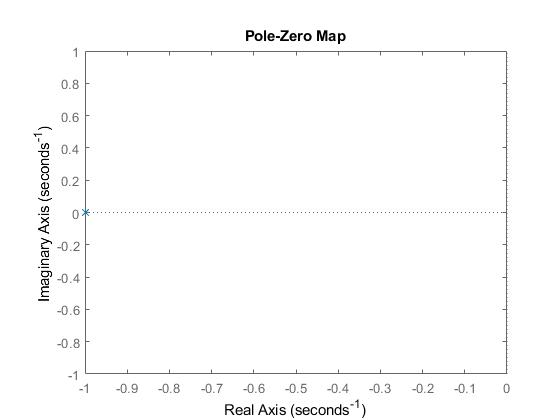
\includegraphics{Imagens/Lab2/tau1.jpg}

Como o pólo da função de transferência se encontra na SPE, conclui-se que o sistema se compartará de uma forma estável.

\hypertarget{parte-2}{%
\paragraph*{Parte 2}\label{parte-2}}
\addcontentsline{toc}{paragraph}{Parte 2}

Para \(\tau = 0.5\), temos a função de transferência dada por
\[
G(S)= \frac {1}{0.5s+1}.
\]

O código implementado no \texttt{Matlab} foi o apresentado abaixo.

\begin{Shaded}
\begin{Highlighting}[]
\VariableTok{g} \OperatorTok{=} \VariableTok{tf}\NormalTok{([}\FloatTok{1}\NormalTok{]}\OperatorTok{,}\NormalTok{ [}\FloatTok{0.5} \FloatTok{1}\NormalTok{])}
\NormalTok{[}\VariableTok{p}\OperatorTok{,} \VariableTok{z}\NormalTok{] }\OperatorTok{=} \VariableTok{pzmap}\NormalTok{(}\VariableTok{g}\NormalTok{)}
\VariableTok{pzmap}\NormalTok{(}\VariableTok{g}\NormalTok{)}
\end{Highlighting}
\end{Shaded}

Tendo como resultados de pólos e zeros:

\begin{verbatim}
p =

    -2


z =

  0×1 empty double column vector
\end{verbatim}

Ou seja, a função de transferência não apresenta zeros e tem seu pólo em \(s = -2\). A sua posição no plano é apresentada na figura abaixo

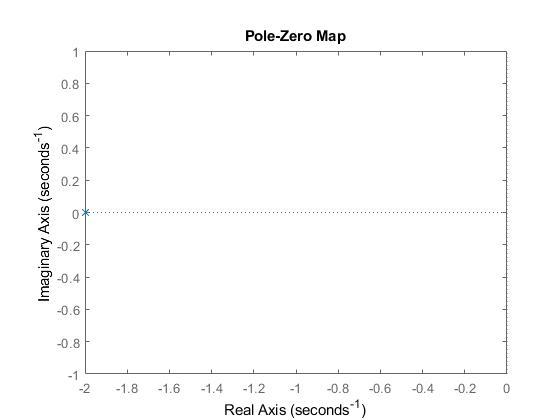
\includegraphics{Imagens/Lab2/tau2.jpg}

Como o pólo da função de transferência se encontra na SPE, conclui-se que o sistema se compartará de uma forma estável. Também é possível concluir que o sistema alcanraça a estabilidade mais rápido para \(\tau = 0.5\).

\hypertarget{parte-3}{%
\paragraph*{Parte 3}\label{parte-3}}
\addcontentsline{toc}{paragraph}{Parte 3}

A simulação do sistema implementada em \texttt{Matlab} está apresentado na figura abaixo.

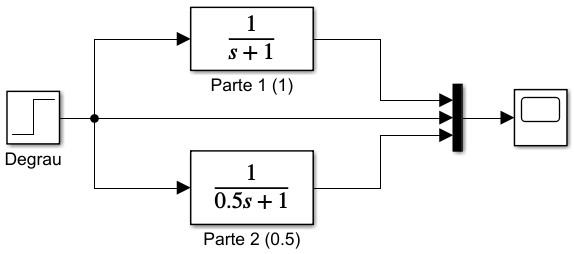
\includegraphics{Imagens/Lab2/sim1.jpg}

O resultado apresentado pelo \emph{scope} é apresentado na figura abaixo.

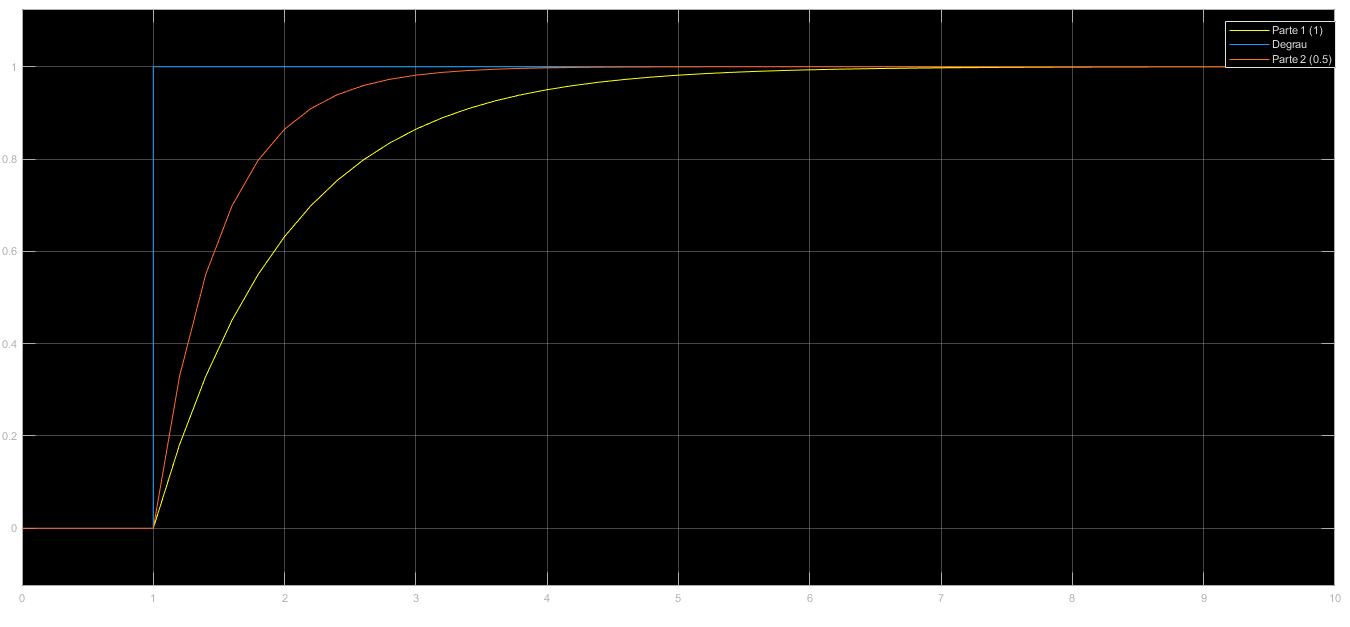
\includegraphics{Imagens/Lab2/resultSim1.jpg}

Percebe-se que, assim como esperado, o sistema se comporta de forma estável e tem uma convergência mais rápida para \(\tau = 0.5\).

\hypertarget{parte-4}{%
\paragraph*{Parte 4}\label{parte-4}}
\addcontentsline{toc}{paragraph}{Parte 4}

Para a última etapa temos a função de transferência dada por
\[
G(S)= \frac {1}{s-1}.
\]

O código implementado no \texttt{Matlab} foi o apresentado abaixo.

\begin{Shaded}
\begin{Highlighting}[]
\VariableTok{g} \OperatorTok{=} \VariableTok{tf}\NormalTok{([}\FloatTok{1}\NormalTok{]}\OperatorTok{,}\NormalTok{ [}\FloatTok{1} \OperatorTok{{-}}\FloatTok{1}\NormalTok{])}
\NormalTok{[}\VariableTok{p}\OperatorTok{,} \VariableTok{z}\NormalTok{] }\OperatorTok{=} \VariableTok{pzmap}\NormalTok{(}\VariableTok{g}\NormalTok{)}
\VariableTok{pzmap}\NormalTok{(}\VariableTok{g}\NormalTok{)}
\end{Highlighting}
\end{Shaded}

Tendo como resultados de pólos e zeros:

\begin{verbatim}
p =

    1


z =

  0×1 empty double column vector
\end{verbatim}

Ou seja, a função de transferência não apresenta zeros e tem seu pólo em \(s = 1\). A sua posição no plano é apresentada na figura abaixo

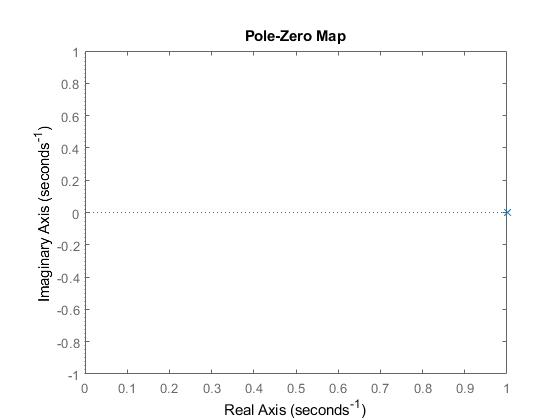
\includegraphics{Imagens/Lab2/tau3.jpg}

Como o pólo da função de transferência se encontra na SPD, conclui-se que o sistema se compartará de uma forma instável. A simulação em \texttt{Matlab} está apresentada na figura abaixo.

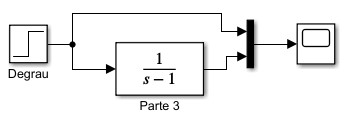
\includegraphics{Imagens/Lab2/sim2.jpg}

O resultado apresentado pelo \emph{scope} é apresentado na figura abaixo.

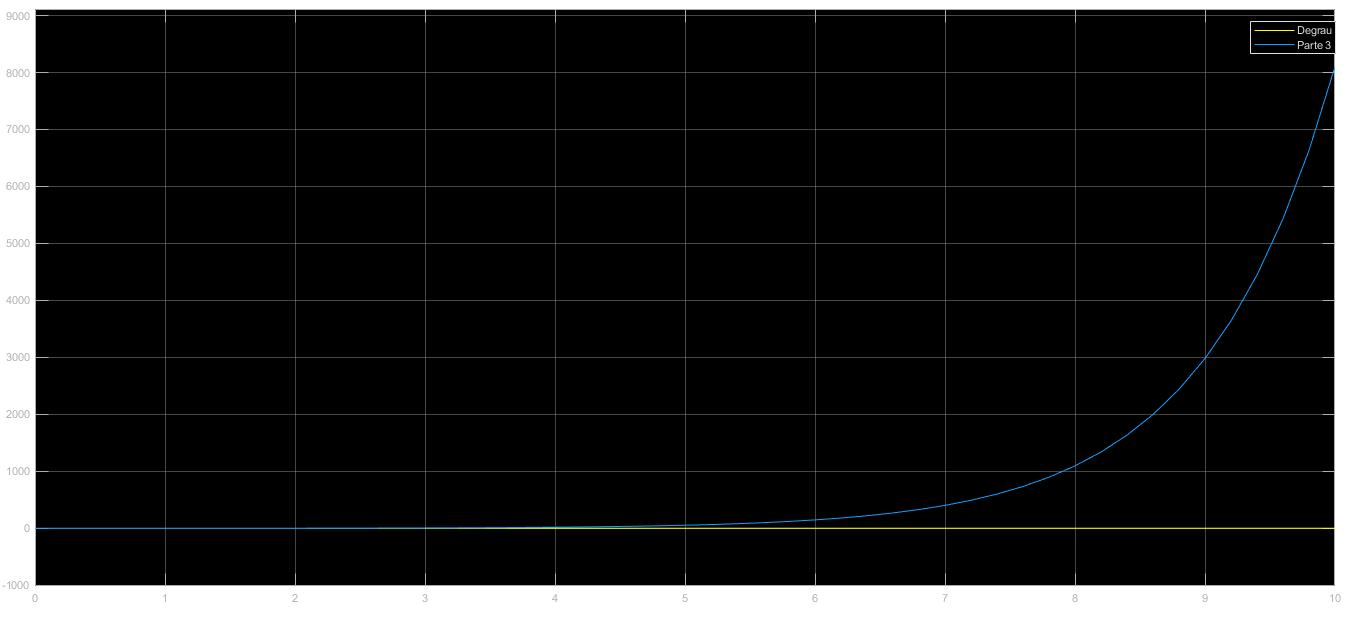
\includegraphics{Imagens/Lab2/resultSim2.jpg}

O resultado comprova o esperado. O sistema se comporta de forma instável para a função de transferência dada por \(G(s) = \frac {1}{s-1}\).

\hypertarget{problema-2}{%
\subsection*{Problema 2}\label{problema-2}}
\addcontentsline{toc}{subsection}{Problema 2}

Considere o sistema de primeira ordem (integrador)
\[
G(s) = \frac {1}{s}.
\]

Determine o pólo e a sua posição no plano \(s\) e simule para uma entrada do tipo degrau unitário e também para \(\sin {(t)}\) (para \(\sin {(t)}\), escolha \textbf{Max Step Size = 0.1} em \textbf{Simulation \(\implies\) Configurarion Parameters}). Note que a saída é a integral da entrada. Tais resultados eram esperados? Dica: relembre que \(Y(s) = G(s)U(s)\), e que se \(x(t) \iff X(S)\), então \(\int_0^t x(\tau) \mathrm{d}\tau \iff X(s)/s\).

\hypertarget{resoluuxe7uxe3o-1}{%
\subsubsection*{Resolução}\label{resoluuxe7uxe3o-1}}
\addcontentsline{toc}{subsubsection}{Resolução}

O código utilizado no \texttt{Matlab} é apresentado abaixo.

\begin{Shaded}
\begin{Highlighting}[]
\VariableTok{g} \OperatorTok{=} \VariableTok{tf}\NormalTok{([}\FloatTok{1}\NormalTok{]}\OperatorTok{,}\NormalTok{ [}\FloatTok{1} \FloatTok{0}\NormalTok{])}
\NormalTok{[}\VariableTok{p}\OperatorTok{,}\VariableTok{z}\NormalTok{] }\OperatorTok{=} \VariableTok{pzmap}\NormalTok{(}\VariableTok{g}\NormalTok{)}
\VariableTok{pzmap}\NormalTok{(}\VariableTok{g}\NormalTok{)}
\end{Highlighting}
\end{Shaded}

Obtendo como resultado:

\begin{verbatim}
p =

     0


z =

  0×1 empty double column vector
\end{verbatim}

Conclue-se então que a função de transferência \(G(s) = \frac {1}{s}\) não tem zeros e tem pólo em \(s = 0\). O mapa da posição no plano é mostrado na figura abaixo.

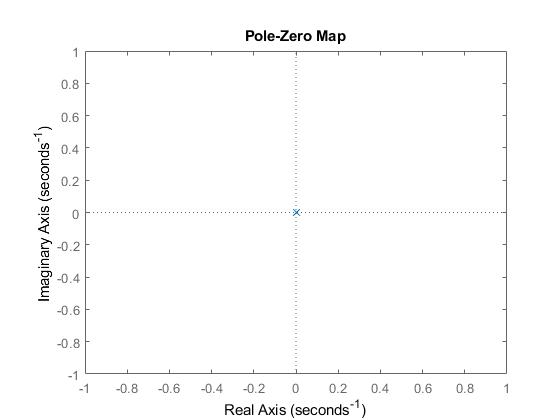
\includegraphics{Imagens/Lab2/prob2.jpg}

Isso mostra que o sistema é um caso crítico. Neste caso a resposta em regime permanente do sistema a uma entrada de amplitude limitada será uma senóide.

A simulação feita em \texttt{Matlab} está apresentada na figura abaixo.

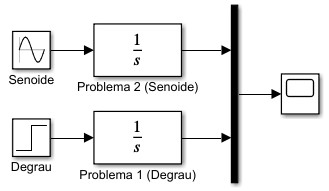
\includegraphics{Imagens/Lab2/simP2.jpg}

O resultado da simulação é apresentado na figura abaixo.

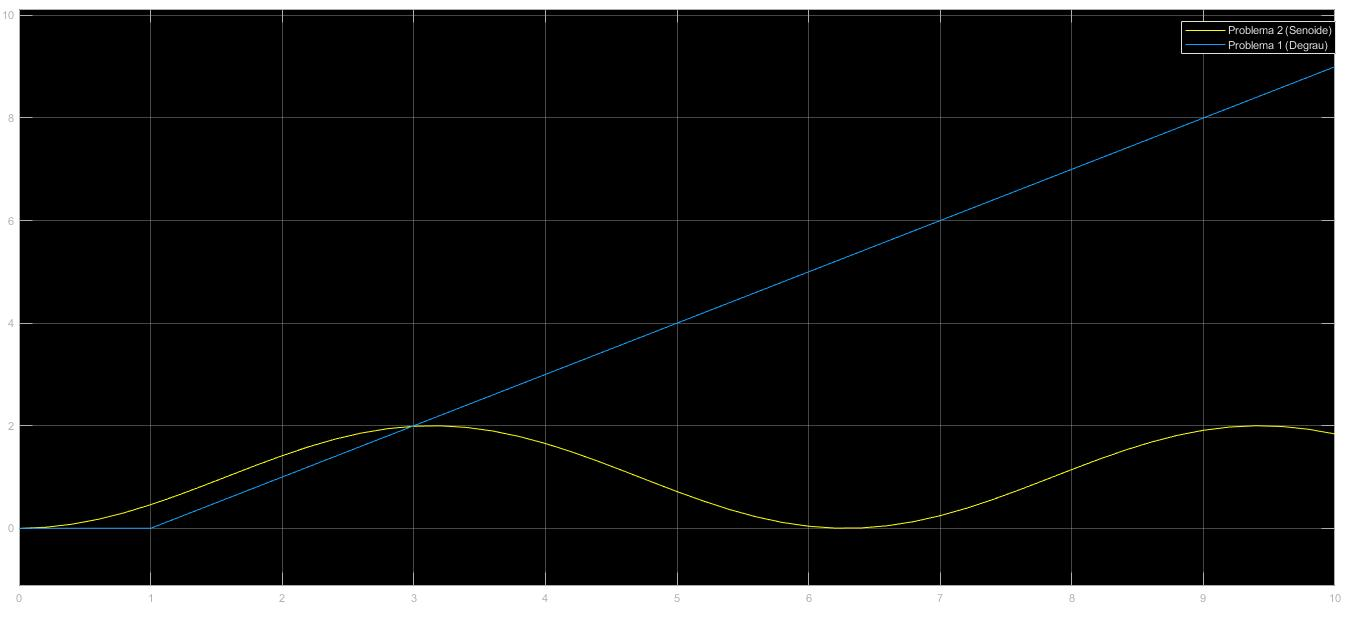
\includegraphics{Imagens/Lab2/prob2B.jpg}

O resultados eram esperados, uma vez que em um estado crítico a função de transferência pode estar em um estado permanente senoidal caso a entrada seja senoidal ou pode divergir caso a entrada seja um sinal constante.

\hypertarget{problema-3}{%
\subsection*{Problema 3}\label{problema-3}}
\addcontentsline{toc}{subsection}{Problema 3}

Considere o sistema de segunda ordem
\[
G(s) = \frac {1}{s^2 +25}.
\]

Determine os pólos e suas posições no plano \(s\). Simule para as seguintes entradas: degrau unitário, \(\sin (4t)\), \(\sin(6t)\). Observe que a saída é limitada. Agora, semule para a entrada \(\sin(5t)\). Note que a amplitude de saída cresce indefinidamente. Tal fenômeno é denominado de \emph{ressonância}. De moro mais geral, para
\[
G(s) = \frac {1}{s^2+\omega_0^2},
\]
teremos ressonância quando aplicamos uma entrada senoidal da forma \(\sin(\omega_0t + \phi)\). Note que a \emph{frequência de ressonância} \(\omega_0\) é igual a parte imaginária dos pólos de \(G(s)\).

\hypertarget{resoluuxe7uxe3o-2}{%
\subsubsection*{Resolução}\label{resoluuxe7uxe3o-2}}
\addcontentsline{toc}{subsubsection}{Resolução}

O código utilizado no \texttt{Matlab} é apresentado abaixo.

\begin{Shaded}
\begin{Highlighting}[]
\VariableTok{g} \OperatorTok{=} \VariableTok{tf}\NormalTok{([}\FloatTok{1}\NormalTok{]}\OperatorTok{,}\NormalTok{ [}\FloatTok{1} \FloatTok{0} \FloatTok{25}\NormalTok{])}
\NormalTok{[}\VariableTok{p}\OperatorTok{,}\VariableTok{z}\NormalTok{] }\OperatorTok{=} \VariableTok{pzmap}\NormalTok{(}\VariableTok{g}\NormalTok{)}
\VariableTok{pzmap}\NormalTok{(}\VariableTok{g}\NormalTok{)}
\end{Highlighting}
\end{Shaded}

Obtendo como resultado:

\begin{verbatim}
p =

   0.0000 + 5.0000i
   0.0000 - 5.0000i


z =

  0×1 empty double column vector
\end{verbatim}

Conclue-se então que a função de transferência \(G(s) = \frac {1}{s^2 +25}\) não tem zeros e tem pólo em \(s = \pm 5i\). O mapa da posição no plano é mostrado na figura abaixo.

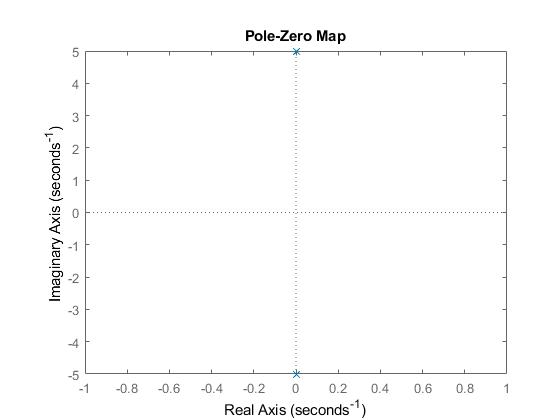
\includegraphics{Imagens/Lab2/prob3.jpg}

De acordo com o mapa de posição, pode-se concluir que a função de transferência é classificada como um caso crítico. A figura abaixo apresenta o modelo de simulação criado no \texttt{Simulink}.

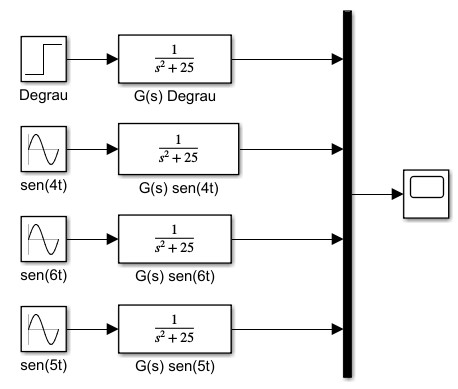
\includegraphics{Imagens/Lab2/modelSim3.jpg}

O resultado da simulação é apresentado abaixo.

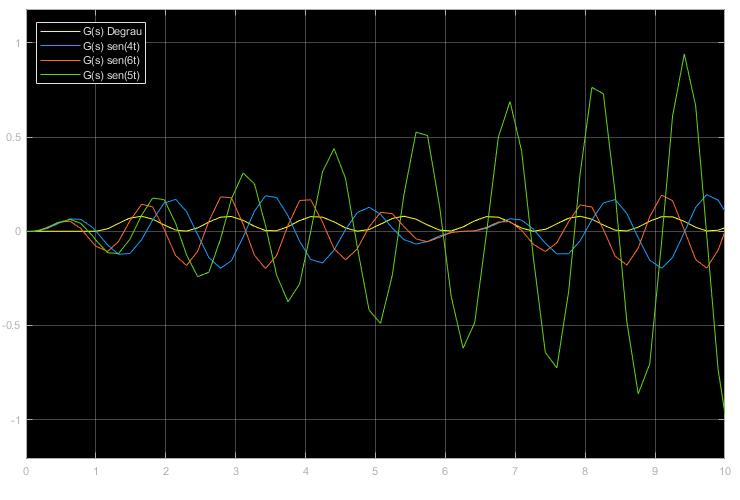
\includegraphics{Imagens/Lab2/prob3Sim.jpg}

É fácil perceber que o modelo se comporta de maneira instável com a entrada \(u(t) = \sin(5t)\), se mostrando estável nas demais situações.

\hypertarget{problema-4}{%
\subsection*{Problema 4}\label{problema-4}}
\addcontentsline{toc}{subsection}{Problema 4}

Considere o sistema de segunda orde
\[
G(s) = \frac {1.6}{(s+1)(s+2)} = \frac {0.8}{0.5s^2+1.5s+1}.
\]

Determine os pólos e suas posições no plano \(s\) e simule para uma entrada do tipo degrau unitário. Note que não há sobressinal. Tal resultado era esperado? Justifique.

Agora, adicionando um zero, temos
\[
G(s) = \frac {1.6(\beta s+1)}{(s+1)(s+2)} = \frac {0.8(\beta s+1)}{0.5s^2 +1.5s +1},
\]
onde \(\beta = 0.1\), \(\beta = 0.6\), \(\beta = 0.99\), \(\beta = 1.2\), \(\beta = 2\), \(\beta = 10\). Para cada valor de \(\beta\), determine os pólos e zeros, suas posições no plano \(s\) e simule para uma entrada do tipo degrau unitário. Analise e compare os resultados. Note que dependendo da posição do zero o sobressinal será maior ou menor, podendo também não estar presente.

\hypertarget{resoluuxe7uxe3o-3}{%
\subsubsection*{Resolução}\label{resoluuxe7uxe3o-3}}
\addcontentsline{toc}{subsubsection}{Resolução}

Utilizando a função \texttt{pzmap()} do \texttt{Matlab} para encontrar os pólos da função de transferência \(G(s) = \frac {0.8}{0.5s^2+1.5s+1}\) temos que a função não possui zeros e possui pólos para \(s = -2\) e \(s = -1\). O mapa de posições é apresentado na figura abaixo.

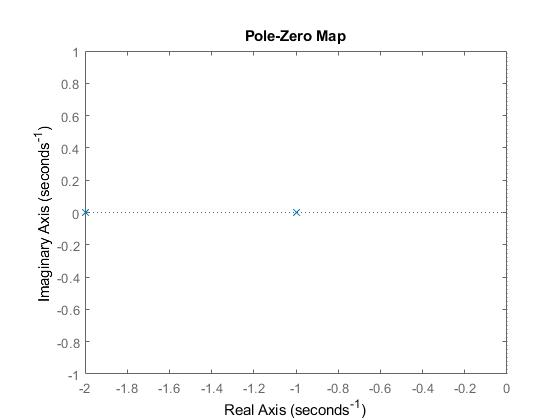
\includegraphics{Imagens/Lab2/prob4.jpg}

O resultado da função de transferência é apresentado na figura abaixo.

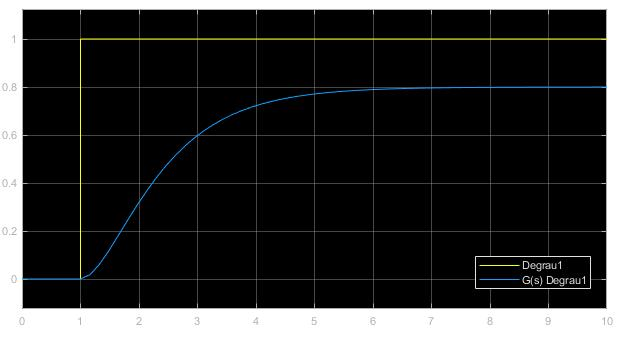
\includegraphics{imagens/Lab2/prob41.jpg}

O resultado não era esperado pois, para uma Função de Transferência de segundo grau é esperado que a resposta tenha sobressinal. Agora, considerando a função de transferência
\[
G(s) = \frac {0.8(\beta s+1)}{0.5s^2+1.5s+1},
\]
e substituindo os valores de \(\beta\) pelos valores propostos temos os valores de zero e pólo apresentados na tabela abaixo.

\begin{table}

\caption{\label{tab:unnamed-chunk-6}Valores de Pólo e Zero variando $\beta$}
\centering
\begin{tabular}[t]{lll}
\toprule
  & Pólos & Zeros\\
\midrule
$\beta = 0.1$ & {-2, -1} & -10.0\\
$\beta = 0.6$ & {-2, -1} & -1.67\\
$\beta = 0.99$ & {-2, -1} & -1.01\\
$\beta = 1.2$ & {-2, -1} & -0.83\\
$\beta = 2$ & {-2, -1} & -0.50\\
\addlinespace
$\beta = 10$ & {-2, -1} & -0.10\\
\bottomrule
\end{tabular}
\end{table}

Os gráficos de posição estão apresentados abaixo.

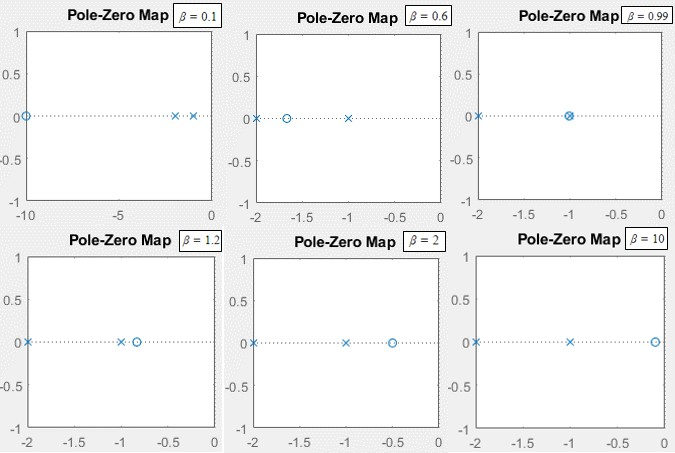
\includegraphics{Imagens/Lab2/prob4Varios.jpg}

A simulação feita em \texttt{Matlab} está apresentada na figura abaixo.

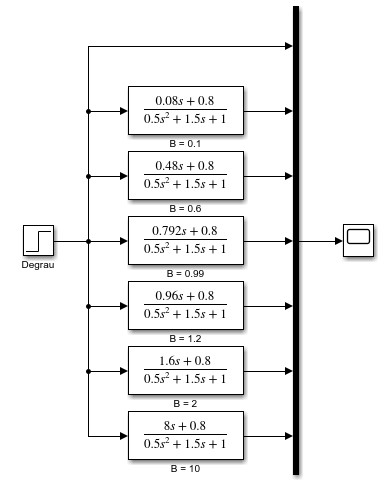
\includegraphics{Imagens/Lab2/modelSim4.jpg}

O resultado da simulação está apresentado na figura abaixo.

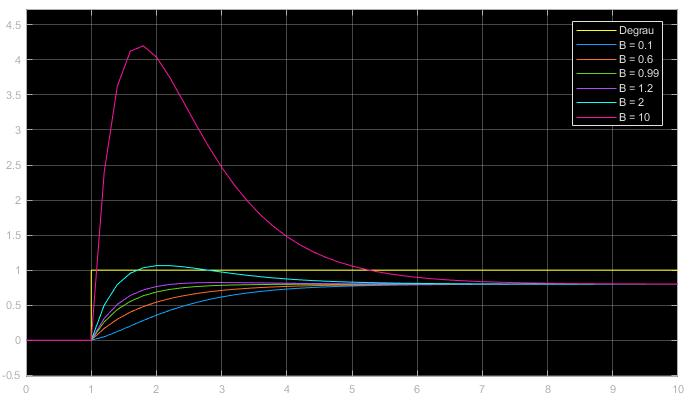
\includegraphics{Imagens/Lab2/prob4SimResult.jpg}

É possível perceber que quanto mais alto o valor de \(\beta\) maior o sobressinal. Também é possível perceber que há um intervalo no qual o tempo de reação aumenta, encontrando seu tempo de reação mínimo, voltando então a aumentar.

\hypertarget{problema-5}{%
\subsection*{Problema 5}\label{problema-5}}
\addcontentsline{toc}{subsection}{Problema 5}

Considere o sistema de segunda ordem
\[
G(s) = \frac {0.9}{s^2+s+1}.
\]

Determine os pólos e suas posições no plano \(s\) e simule para uma entrada do tipo degrau unitário. Note que há sobressinal. Tal resultado era esperado? Justifique.

Agora, adicionando um zero, temos
\[
G_z(s) = \frac {0.9(\beta s+1)}{s^2+s+1},
\]
onde \(\beta = 0.05\), \(\beta = 0.5\), \(\beta = 1\) e \(\beta = 2.5\). Para cada valor de \(\beta\) determine os pólos e zeros, suas posições no plano \(s\) e simule para uma entrada do tipo degrau unitário. Analise e compare os resultados.

\hypertarget{resoluuxe7uxe3o-4}{%
\subsubsection*{Resolução}\label{resoluuxe7uxe3o-4}}
\addcontentsline{toc}{subsubsection}{Resolução}

Utilizando a função \texttt{pzmap()} do \texttt{Matlab} para encontrar os pólos da função de transferência \(G(s) = \frac {0.9}{s^2+s+1}\) temos que a função não possui zeros e possui pólos para \(s = -0.5 + 0.86i\) e \(s = -0.5 -0.86i\). O mapa de posições é apresentado na figura abaixo.

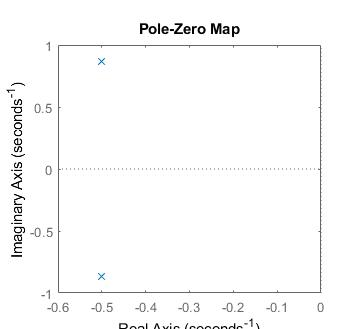
\includegraphics{Imagens/Lab2/prob5.jpg}

O resultado da função de transferência é apresentado na figura abaixo.

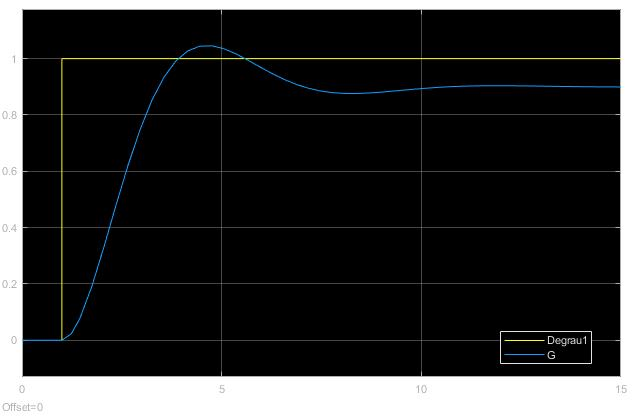
\includegraphics{imagens/Lab2/prob5Sim.jpg}

É possível perceber que há sobressinal.

Agora, considerando a função de transferência \(G_z(s) = \frac {0.9(\beta s+1)}{s^2+s+1}\), e substituindo os valores de \(\beta\) pelos valores propostos temos os valores de zero e pólo apresentados na tabela abaixo.

\begin{table}

\caption{\label{tab:unnamed-chunk-7}Valores de Pólo e Zero variando $\beta$}
\centering
\begin{tabular}[t]{lll}
\toprule
  & Pólos & Zeros\\
\midrule
$\beta = 0.05$ & {$-0.5 \pm 0.86i$} & -20.0\\
$\beta = 0.5$ & {$-0.5 \pm 0.86i$} & -2.0\\
$\beta = 1$ & {$-0.5 \pm 0.86i$} & -1.0\\
$\beta = 2.5$ & {$-0.5 \pm 0.86i$} & -0.4\\
\bottomrule
\end{tabular}
\end{table}

Os gráficos de posição estão apresentados abaixo.

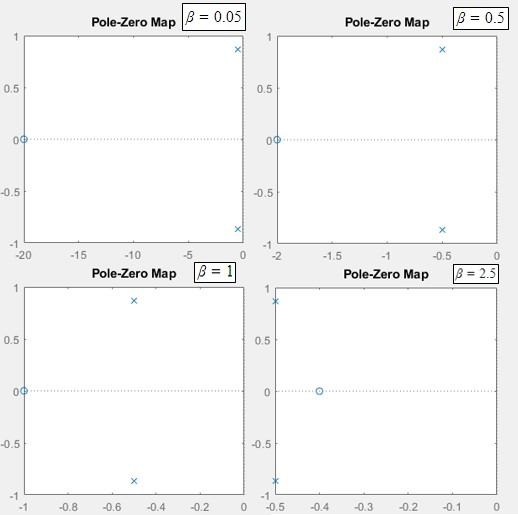
\includegraphics{Imagens/Lab2/prob5Varios.jpg}

A simulação feita em \texttt{Matlab} está apresentada na figura abaixo.

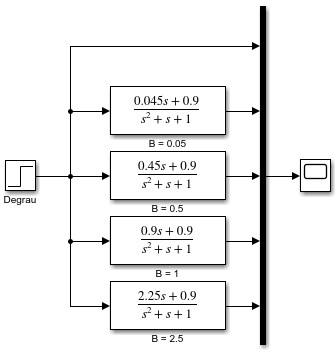
\includegraphics{Imagens/Lab2/modelSim5.jpg}

O resultado da simulação está apresentado na figura abaixo.

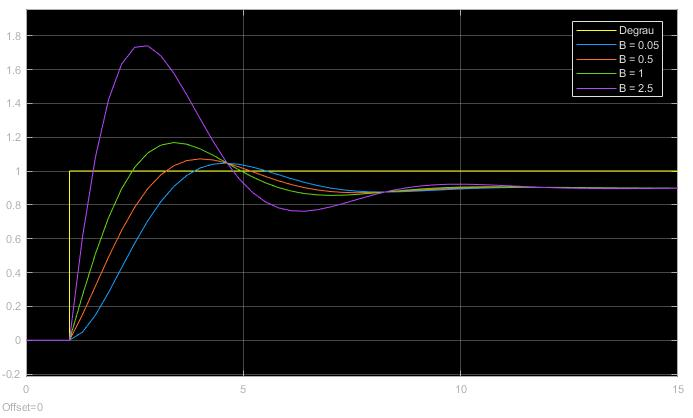
\includegraphics{Imagens/Lab2/prob5SimResult.jpg}

É possível perceber que quanto mais alto o valor de \(\beta\) maior o sobressinal e o tempo de resposta do sistema.

\hypertarget{problema-6}{%
\subsection*{Problema 6}\label{problema-6}}
\addcontentsline{toc}{subsection}{Problema 6}

Considere o sistema de segunda ordem de fase não-mínima
\[
G(s) = \frac {-s+1}{0.5s^2+1.5s+1}.
\]

Determine os pólos e o zero, suas posições no plano \(s\) e simule para uma entrada do tipo degrau unitário. Note que a resposta é negativa nos instantes iniciais. Justificaremos tal comportamento no que se segue.

Escrevemos
\[
G(s) = \frac {-s+1}{0.5s^2+1.5s+1} = \overbrace{\frac {1}{0.5s^2+1.5s+1}}^{G_1(s)} - \overbrace{\frac {s}{0.5s^2+1.5s+1}}^{G_2(s) = sG_1(S)}.
\]

Assim,
\[
Y(s) = G(s)U(s) = G_1(s)U(s)-G_2(s)U(s) = \underbrace{G_1(s)U(s)}_{Y_1(s)} - \underbrace{sG_1(s)U(s)}_{Y_2(s) = sY_1(s)}.
\]

Relembre-se que se \(x(t) \iff X(S)\) com \(x(0) = 0\), então \(dx(t)/dt \iff sX(s)\). Portanto,
\[
y(t) = y_1(t)-y_2(t)=y_1(t)- \frac {dy_1(t)}{dt}.
\]

Verifique a validade da equação acima no Simulink (utilize o bloco \textbf{Derivative} no Simulink) para uma entrada do tipo degrau unitário. Analise o motivo da resposta ser negativa nos instantes iniciais.

\hypertarget{resoluuxe7uxe3o-5}{%
\subsubsection*{Resolução}\label{resoluuxe7uxe3o-5}}
\addcontentsline{toc}{subsubsection}{Resolução}

Utilizando a função \texttt{pzmap()} do \texttt{Matlab} para encontrar os pólos da função de transferência \(G(s) = \frac {-s +1}{0.5s^2+1.5s+1}\) temos que a função possui zeros para \(s=1\) e possui pólos para \(s = -2\) e \(s = -1\). O mapa de posições é apresentado na figura abaixo.

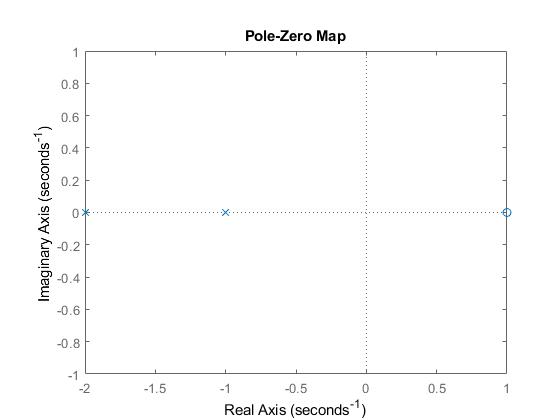
\includegraphics{Imagens/Lab2/prob6A.jpg}

A resposta de \(G(s)\) a uma função degrau unitário é apresentada na figura abaixo.

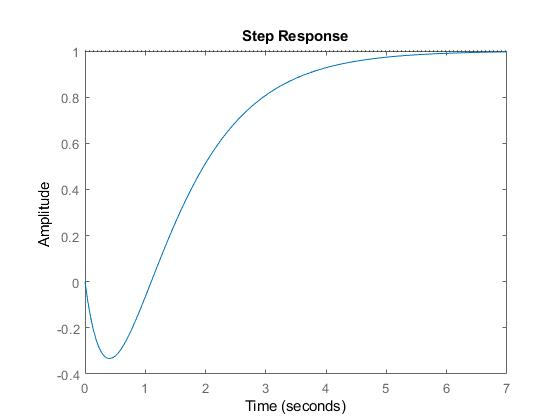
\includegraphics{Imagens/Lab2/prob6B.jpg}

A validade da equação proposta pelo programa é apresentada na figura abaixo. Pode-se perceber que a equação é valida pois as curvas são satisfatoriamente similares.

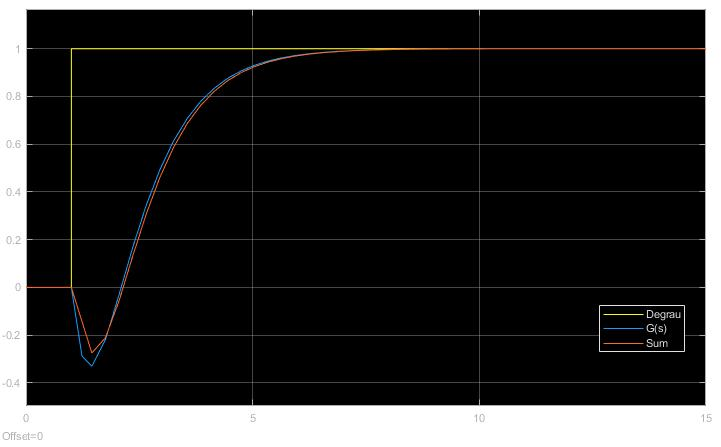
\includegraphics{Imagens/Lab2/prob6C.jpg}

O motivo da resposta ser negativa se deve ao fato de o zero da função \(G(s)\) se encontrar no SPD.

\hypertarget{identificauxe7uxe3o-de-sistemas}{%
\chapter{Identificação de Sistemas}\label{identificauxe7uxe3o-de-sistemas}}

\hypertarget{apresentauxe7uxe3o-do-laboratuxf3rio-1}{%
\section{Apresentação do Laboratório}\label{apresentauxe7uxe3o-do-laboratuxf3rio-1}}

\hypertarget{objetivo-1}{%
\subsection{Objetivo}\label{objetivo-1}}

Nesta experiência, veremos como modelar matematicamente um sistema linear por uma Função de Transferência. Identificaremos os parâmetros de uma Função de Transferência de primeira e de segunda ordem. Compararemos a dinâmica do sistema com a do modelo matemático.

\hypertarget{modelagem-de-sistemas-lineares}{%
\subsection{Modelagem de Sistemas Lineares}\label{modelagem-de-sistemas-lineares}}

Encontrar um modelo matemático que capture as características dinâmicas relevantes de um sistema real é de fundamental importância para a análise e controle do sistema. No Laboratório 1 estudamos um modelo linear com motor CC. Tal modelo pode ser obtido a partir das leis da física (mecânica e eletromagnetismo) e os valores dos parâmetros dependem de constantes e coeficientes físicos (indutância do enrolamento, resistência do enrolamento, constante de torque do motor, coeficiente de atrito ciscoso). Em situações reais, não conheceremos uma estimativa para os mesmos. Por exemplo, todo resistor possui um valor normal e uma faixa de tolerância percentual (e.g.~\(R = 100 \Omega \pm 5\%\)). Além disso, muitas vezes a determinação de um modelo matemático para um sistema a partir de leis naturais é extremamente difícil e, mesmo no caso em que isso é possível, o modelo obtido pode ser demasiadamente complexo para ser estudado matematicamente.

Devido às dificuldades que acabamos de expor, em geral buscamos um modelo matemático relativamente simples mas que capture, ao menos aproximadamente, as características dinâmicas relevantes do sistema. Assim, primeiramente fixamos um modelo (\emph{modelagem} do sistema) e em seguida determinamos de maneira aproximada o valor de seus parâmetros (\emph{identificação} dos parâmetros).

Nesta experiência, consideraremos apenas sistemas lineares que possam ser modelados por uma função de Transferência \(G(s)\) de primeira ordem ou de segunda ordem. Veremos então como identificar os parâmetros de \(G(s)\).

\hypertarget{identificauxe7uxe3o-de-sistemas-de-primeira-ordem}{%
\subsection{Identificação de sistemas de primeira ordem}\label{identificauxe7uxe3o-de-sistemas-de-primeira-ordem}}

Toda Função de Transferência \(G(s)\) de primeira ordem pode ser escrita na forma padrão como

\begin{align}
G(s) = \frac{K}{\tau s+1}. \label{eq:eq31}
\end{align}

Supunha que \(G(s)\) é estável, ou seja, \(\tau > 0\). considere uma entrada \(u(t) = A\) do tipo degrau de magnitude \(A\). Temos que a saída correspondente é
\[
y(t) = AK(1- e^{\frac {-t}{\tau}}).
\]

O valor da saída em regime permanente é
\[
y(\infty) = AK,
\]
e o tempo de acomodação de \(5\%\) é dado por
\[
0.95KA = KA(1- e^{\frac {-t_s(5\%)}{\tau}}) \implies t_s(5\%) =3 \tau.
\]

Isto é ilustrado na figura 1.

\begin{figure}
\centering
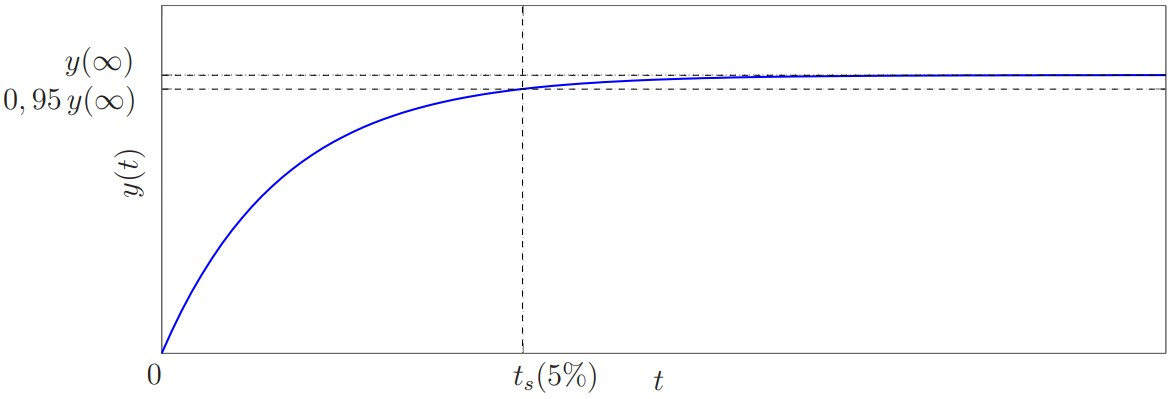
\includegraphics{Imagens/Lab3/Explicação/fig1.jpg}
\caption{Figura 1: Resposta de um sistema de primeira ordem ao degrau.}
\end{figure}

Logo,

\begin{align}
K = \frac{y(\infty)}{A},  \tau = \frac {t_s(5\%)}{3}. \label{eq:eq32}
\end{align}

\hypertarget{identificauxe7uxe3o-de-sistemas-de-segunda-ordem}{%
\subsection{Identificação de Sistemas de Segunda Ordem}\label{identificauxe7uxe3o-de-sistemas-de-segunda-ordem}}

Toda Função de Transferência \(G(s)\) de segunda ordem com pólos não-nulos pode ser escrita como

\begin{align}
G(s) = \frac {K \omega_n^2}{s^2+2\xi \omega_n+ \omega_n^2}, \label{eq:eq33}
\end{align}

onde \(\omega_n > 0\). Os pólos de \(G(s)\) são:
\[
p_{1,2} = - \xi \omega_n \pm \sqrt{\xi^2 -1}.
\]

Temos as seguintes situações:

\begin{enumerate}
\def\labelenumi{\arabic{enumi}.}
\tightlist
\item
  Sistema não-amortecido (\(\xi = 0\)): os pólos são complexos com \(p_{1,2} = \pm j \omega_n\), e a resposta a uma entrada do tipo degrau é senoidal.
\item
  Sistema sub-amortecido (\(0< \xi <1\)): os pólos são complexos com \(p_{1,2} = - \xi \omega_n \pm j \omega_n\sqrt{1 - \xi^2}\) e a resposta ao degrau apresenta oscilação e sobressinal.
\item
  Sistema criticamente amortecido (\(\xi = 1\)): os pólos são reais e iguais com \(p_{1,2} = -\xi \omega_n\) e a resposta ao degrau não apresenta oscilação nem sobressinal.
\item
  Sistema super-amortecido (\(\xi >1\)): os pólos são reais, negativos e diferentes e a resposta ao degrau não apresenta oscilação nem sobressinal.
\item
  Sistema instável (\(\xi < 0\)): os pólos possuem parte real positiva.
\end{enumerate}

\hypertarget{sistemas-sub-amortecidos}{%
\subsubsection{Sistemas sub-amortecidos}\label{sistemas-sub-amortecidos}}

Suponha que \(G(s)\) é estável com \(0 < \xi < 1\) (sub-amortecido). Considere uma entrada \(u(t) = A\) do tipo degrau de magnitude \(A\). A resposta correspondente \(y(t)\) é ilustrada na figura 2.

\begin{figure}
\centering
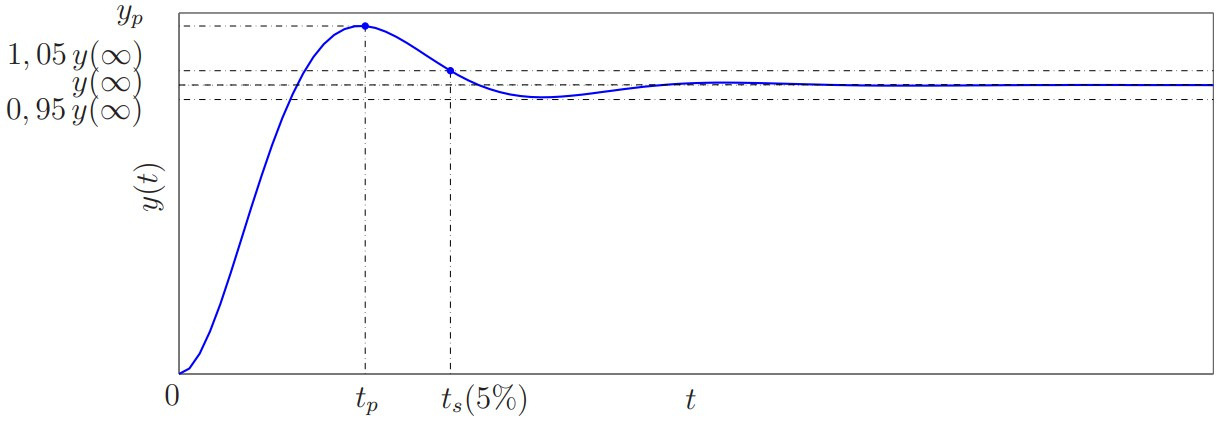
\includegraphics{Imagens/Lab3/Explicação/fig2.jpg}
\caption{Figura 2: Resposta de um sistema de segunda ordem sub-amortecido ao degrau.}
\end{figure}

Temos que
\[
y(\infty) = KA, \quad M_p= \frac {y_p-y(\infty)}{y(\infty)} = e^{\frac {-(\xi \pi)}{\sqrt{1-\xi^2}}}, \quad
t_p = \frac {\pi}{\omega_n\sqrt{1-\xi^2}}.
\]

Logo,

\begin{align}
K = \frac {y(\infty)}{A}, \quad M_p = \frac {y_p - y(\infty)}{y(\infty)}, \quad \xi = \sqrt{\frac {(\ln{M_p})^2}{(\ln{M_p})^2+\pi^2}}, \quad \omega_n = \frac {\pi}{t_p\sqrt{1-\xi^2}}.  \label{eq:eq34}
\end{align}

\hypertarget{sistemas-criticamente-amortecidos-e-super-amortecidos}{%
\subsubsection{Sistemas criticamente amortecidos e super-amortecidos}\label{sistemas-criticamente-amortecidos-e-super-amortecidos}}

Suponha que \(G(s)\) é estável com \(\xi \geq 1\) (criticamente amortecido ou super-amortecido). Neste caso, os dois pólos de \(G(s)\) são reais e a resposta ao degrau se assemelha ao de um sistema de primeira ordem (não apresenta oscilação nem sobressinal). Podemos identificar \(G(s)\) indiretamente através da identificação da Função de Transferência \(F(s)\) em malha-fechada. Considere o diagrama de blocos em malha-fechada mostrando na Figura 3, onde \(K_c > 0\) é o ganho de um controlador proporcional e \(r\) é a referência.

\begin{figure}
\centering
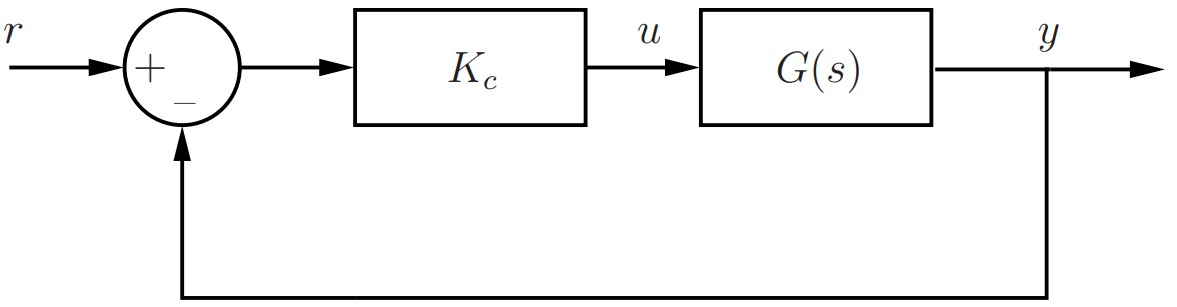
\includegraphics{Imagens/Lab3/Explicação/fig3.jpg}
\caption{Figura 3: Diagrama de blocos em malha-fechada.}
\end{figure}

Relembre que
\[
F(s) = \frac {Y(s)}{R(s)} = \frac {K_cG(s)}{1+K_cG(s)}.
\]

Para qualquer \(K_c > 0\), temos que \(F(s)\) é um sistema de segunda ordem estável. E, quando \(K_c > 0\) for suficientemente grade, temos que \(F(s)\) será um sistema de segunda ordem sub-amortecido. Assim, escolhemos \(K_c\) de modo que \(F(s)\) seja sub-amortecido e então identificamos \(F(s)\) conforme descrito na seção anterior aplicando uma referência \(r(t) = A\) do tipo degrau de magnitude \(A\). Desta maneira, identificaremos \(G(s)\) indiretamente pois

\begin{align}
F(s) = \frac {K_cG(s)}{1+K_cG(s)} \implies G(s) = \frac {F(s)}{K_c - K_cF(s)}.  \label{eq:eq35}
\end{align}

\hypertarget{procedimentos-1}{%
\section{Procedimentos}\label{procedimentos-1}}

\hypertarget{problema-1-1}{%
\subsection*{Problema 1}\label{problema-1-1}}
\addcontentsline{toc}{subsection}{Problema 1}

Aplique um degrau \(u(t) = 2\) no Sistema 1 do arquivo \texttt{MatLab3.mdl} do Simulink. Pelas características da resposta, modele o Sistema 1 como uma Função de Transferência \(G_1(s)%
\) de primeira ou segunda ordem. Em seguida, identifique os parâmetros do modelo utilizando a equação \eqref{eq:eq32} ou \eqref{eq:eq34}. Compare a resposta do modelo identificado com a do Sistema 1.

\hypertarget{resoluuxe7uxe3o-6}{%
\subsubsection*{Resolução}\label{resoluuxe7uxe3o-6}}
\addcontentsline{toc}{subsubsection}{Resolução}

Simulando o sistema do modelo 1 obtemos o resultado abaixo.

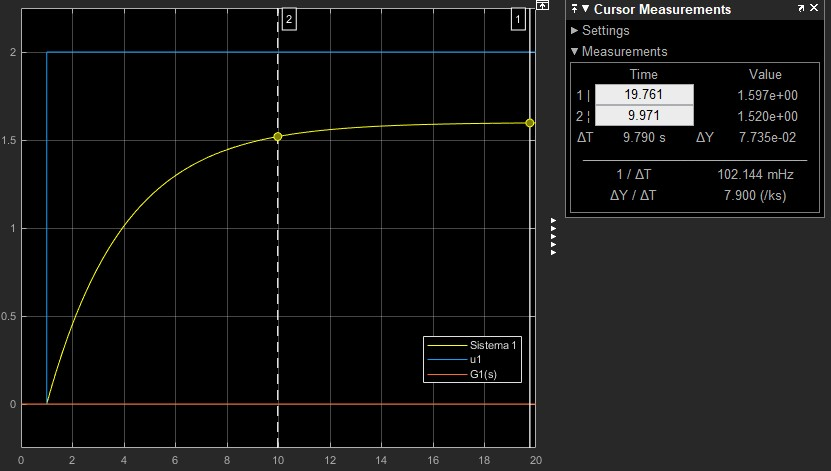
\includegraphics{Imagens/Lab3/Resolução/prob1A.jpg}

Pela curva feita espera-se que a Função de Transferência seja de primeira ordem. Utilizando as ferramentas fornecidas pelo \texttt{Simulink} foi estimado que
\[
y(\infty) = 1.6 \\
0.95y(\infty) = 1.52 \implies  t_s(5\%) = 9.97s \implies \tau = 3.33
\]

Assim,
\[
G_1(s) = \frac {0.8}{3.33s+1}.
\]

Simulando \(G_1(s)\), temos o resultado apresentado abaixo.

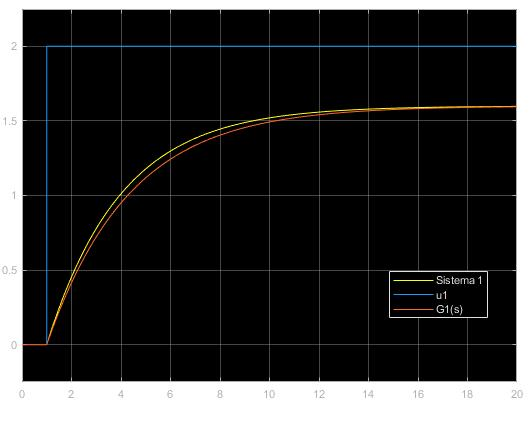
\includegraphics{Imagens/Lab3/Resolução/prob1B.jpg}

Percebe-se, assim, que a Função de Transferência \(G_1(s)\) se aproxima satisfatoriamente bem do Sistema 1.

\hypertarget{problema-2-1}{%
\subsection*{Problema 2}\label{problema-2-1}}
\addcontentsline{toc}{subsection}{Problema 2}

Aplique um degrau \(u(t) = 4\) no Sistema 2. Pelas características da resposta modele o Sistema 2 como uma Função de Transferência \(G_2(s)\) de primeira ou segunda ordem. Em seguida, identifique os parâmetros do modelo utilizando a equação \eqref{eq:eq32} ou \eqref{eq:eq34}. Realize os cálculos na linha de comando do \texttt{Matlab} (\(\ln{(x)} \implies \log{(x)}\) e \(\sqrt{x} \implies \text{sqrt(x)}\)).Compare a resposta do modelo identificando com a do Sistema 2.

\hypertarget{resoluuxe7uxe3o-7}{%
\subsubsection*{Resolução}\label{resoluuxe7uxe3o-7}}
\addcontentsline{toc}{subsubsection}{Resolução}

Simulando o sistema do modelo 1 obtemos o resultado abaixo.

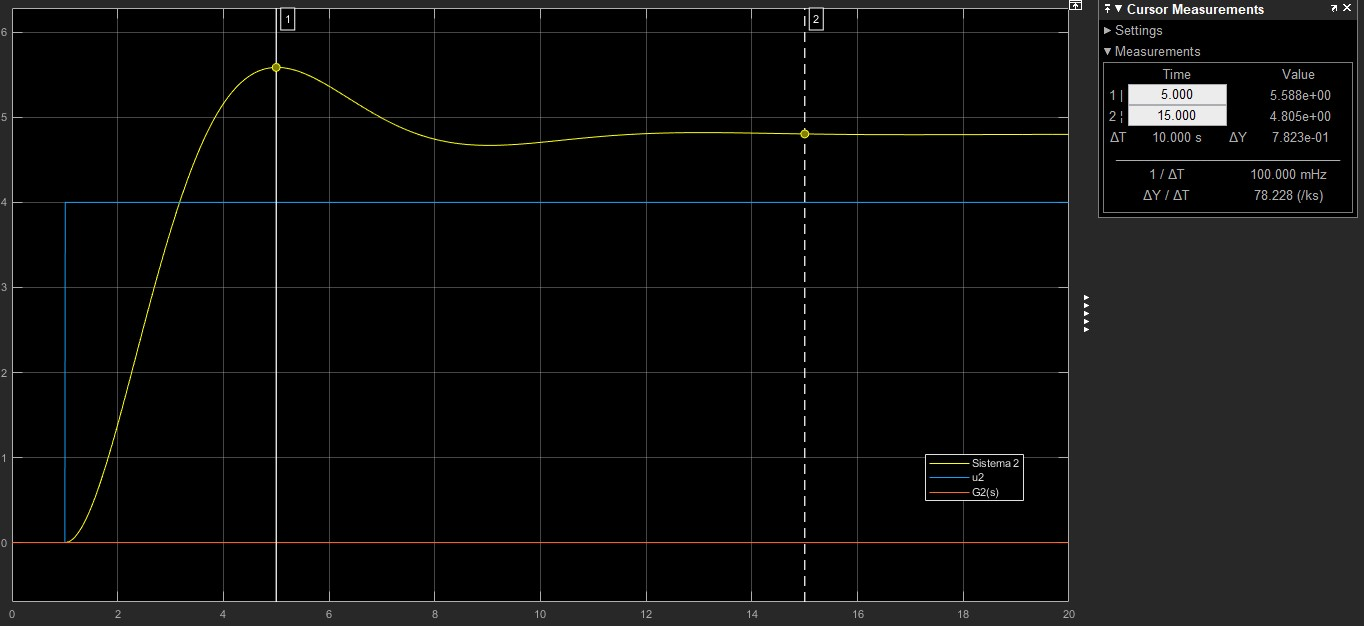
\includegraphics{Imagens/Lab3/Resolução/prob2A.jpg}

Pela curva feita espera-se que a Função de Transferência seja de segunda ordem. Utilizando as ferramentas fornecidas pelo \texttt{Simulink} foi estimado que
\[
y_p = 5.588\\
y(\infty) = 4.805 \\
t_p = 5s
\]

Dessa forma, aplicando as equações 3.4, temos que
\[
K = 1.2, \quad M_p = 0.163, \quad \xi = 0.5 \quad \text{e} \quad \omega_n = 0.7255.
\]

Dessa forma, a Função de Transferência \(G_2(s)\) será
\[
G_2(s) = \frac {0.6316}{s^2 + 0.7255s + 0.5264}.
\]
Simulando \(G_2(s)\), temos o resultado apresentado abaixo.

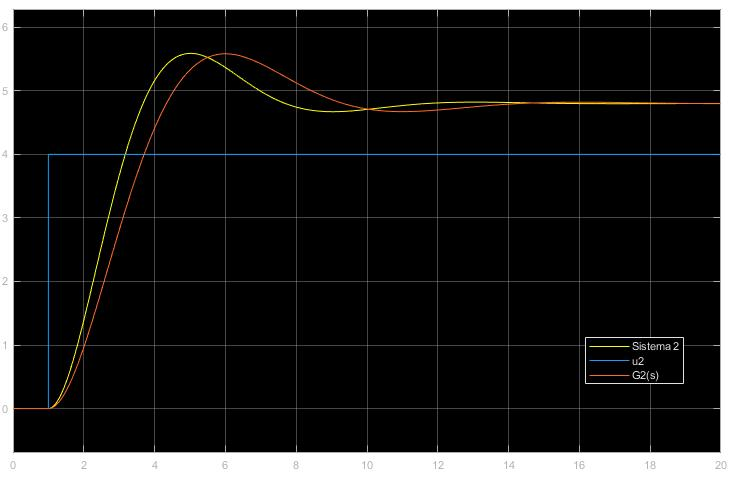
\includegraphics{Imagens/Lab3/Resolução/prob2B.jpg}

Percebe-se, assim, que a Função de Transferência \(G_2(s)\) se assemelha ao Sistema 2,porém, com menor precisão que a função \(G_1(s)\) se aproximou do Sistema 2.

\hypertarget{problema-3-1}{%
\subsection*{Problema 3}\label{problema-3-1}}
\addcontentsline{toc}{subsection}{Problema 3}

\hypertarget{parte-a}{%
\subsubsection*{Parte A}\label{parte-a}}
\addcontentsline{toc}{subsubsection}{Parte A}

Aplique um degrau \(u(t) = 3\) no Sistema 3. Obtenha um modelo aproximado para o Sistema 3 como uma Função de Transferência \(G(s)\) de primeira ordem. Agora implemente o diagrama de blocos em malha fechada da Figura 3 para o Sistema 3 com \(r(t) = 1\) do tipo degrau e \(K_c = 3\)Observamos que, na Figura 3, se \(G(s)\) é de primeira ordem, então a Função de Transferência em malha fechada \(F(s)\) também será de primeira ordem para qualquer valor de \(K_c > 0\). A resposta do Sistema 3 em malha-fechada está de acordo com tal propriedade? O que pode estar errado?

\hypertarget{resoluuxe7uxe3o-8}{%
\paragraph*{Resolução}\label{resoluuxe7uxe3o-8}}
\addcontentsline{toc}{paragraph}{Resolução}

Simulando o sistema do modelo 1 obtemos o resultado abaixo.

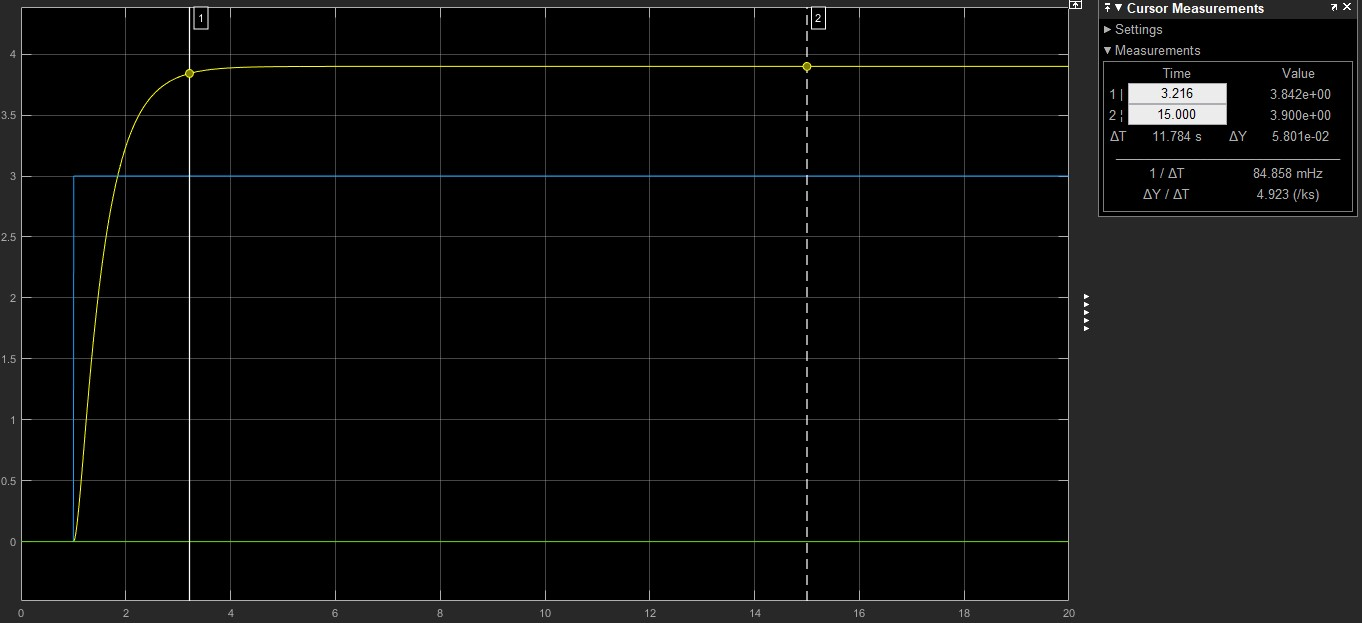
\includegraphics{Imagens/Lab3/Resolução/prob3AA.jpg}

Pela curva feita espera-se que a Função de Transferência seja de primeira ordem. Utilizando as ferramentas fornecidas pelo \texttt{Simulink} foi estimado que
\[
y(\infty) = 3.9 \\
0.95y(\infty) = 3.8415 \implies  t_s(5\%) = 3.22s \implies \tau = 1.072
\]

Assim,
\[
G_3(s) = \frac {1.3}{1.072s+1}.
\]

Simulando \(G_1(s)\), temos o resultado apresentado abaixo.

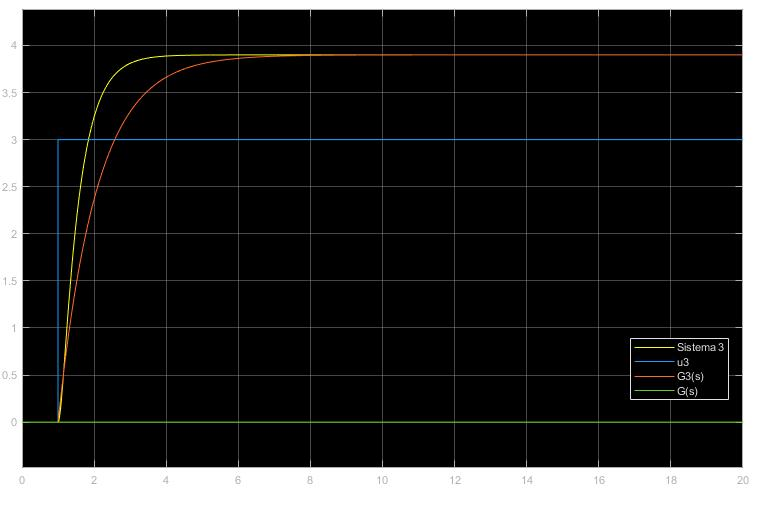
\includegraphics{Imagens/Lab3/Resolução/prob3AB.jpg}

Percebe-se, assim, que a Função de Transferência \(G_B(s)\) não se aproxima satisfatoriamente bem ao Sistema 3. Aplicando a malha fechada vista na figura 3, temos o resultado apresentado abaixo.

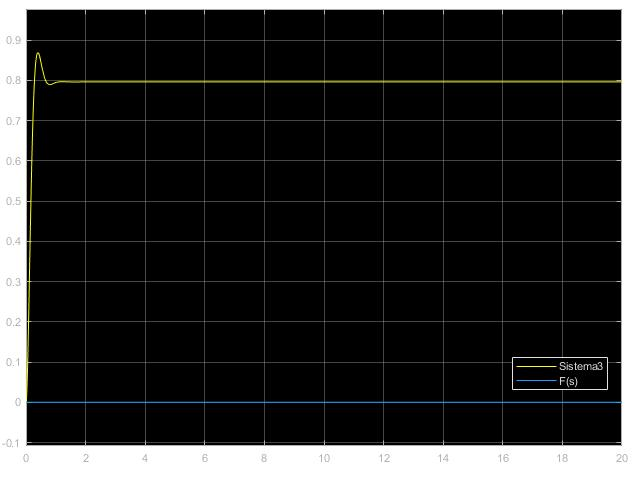
\includegraphics{Imagens/Lab3/Resolução/prob3AC.jpg}

Como \(K_c = 3 > 0\) e a Função de Transferência em malha fechada retornou um sistema de segunda ordem, percebe-se a resposta não está de acordo com a propriedade estabelecida. Desta forma, presume-se que \(G(s)\) não é de primeira ordem e sim de segunda.

\hypertarget{parte-b}{%
\subsubsection*{Parte B}\label{parte-b}}
\addcontentsline{toc}{subsubsection}{Parte B}

Identifique \(F(s)\). Em seguida, identifique \(G(s)\)indiretamente através da equação \eqref{eq:eq55}. Para isto, utilize os seguintes comandos no \texttt{Matlab}:

\begin{Shaded}
\begin{Highlighting}[]
\VariableTok{F} \OperatorTok{=} \VariableTok{tf}\NormalTok{([}\VariableTok{K}\OperatorTok{*}\VariableTok{wn}\OperatorTok{\^{}}\FloatTok{2}\NormalTok{]}\OperatorTok{,}\NormalTok{ [}\FloatTok{1} \FloatTok{2}\OperatorTok{*}\VariableTok{ksi}\OperatorTok{*}\VariableTok{wn} \VariableTok{wn}\OperatorTok{\^{}}\FloatTok{2}\NormalTok{])}
\VariableTok{G} \OperatorTok{=} \VariableTok{F}\OperatorTok{/}\NormalTok{(}\VariableTok{Kc}\OperatorTok{{-}}\VariableTok{Kc}\OperatorTok{*}\VariableTok{F}\NormalTok{)}
\VariableTok{G} \OperatorTok{=} \VariableTok{zpk}\NormalTok{(}\VariableTok{minreal}\NormalTok{(}\VariableTok{G}\NormalTok{)) }\CommentTok{\% minreal simplifica e zpk fatora}
\end{Highlighting}
\end{Shaded}

Note que \(G(s)\) é de segunda ordem com pólos reais. Neste momento, temos condições de responderm o que estava errado em nossa modelagem inicial do Sistema 3 como um sistema de primeira ordem. Compare a resposta em malha-aberta de \(G(s)\) (identificando indiretamente) com a do Sistema 3 para \(u(t) = 3\) do tipo degrau.

\hypertarget{resoluuxe7uxe3o-9}{%
\paragraph*{Resolução}\label{resoluuxe7uxe3o-9}}
\addcontentsline{toc}{paragraph}{Resolução}

Simulando o sistema do Sistema 3 em malha fechada e utilizando as ferramentas fornecidas pelo \texttt{Simulink} foi estimado que
\[
y_p = 0.868 \\
y(\infty) = 0.796 \\
t_p = 0.4s
\]

Assim, tem-se que:
\[
K = 0.796, \quad M_p = 0.09, \quad \xi = 0.61 \quad \text{e} \quad \omega_n= 9.888.
\]

Dessa forma, tem-se que
\[
F(s) = \frac {77.83}{s^2+ 12.01s +97.77}
\]
que gera a curva abaixo.

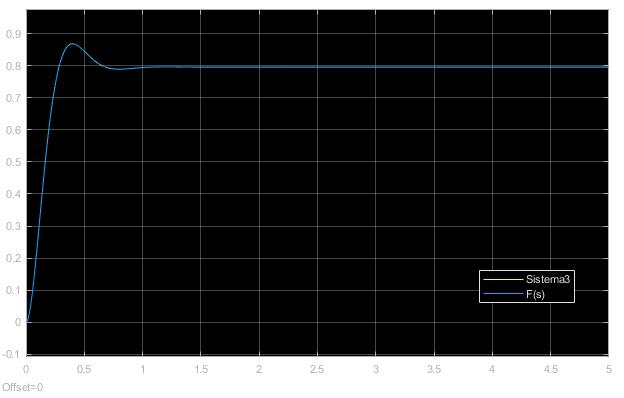
\includegraphics{Imagens/Lab3/Resolução/prob3BA.jpg}

Assim, é possível calcular \(G(s)\) a partir de \(F(s)\), tendo como resultado
\[
G(s) = \frac {25.94}{s^2+12.025s+19.96}.
\]

Agora é possível comprar \(G(s)\) com sua curva anterior, gerando o resultado abaixo.

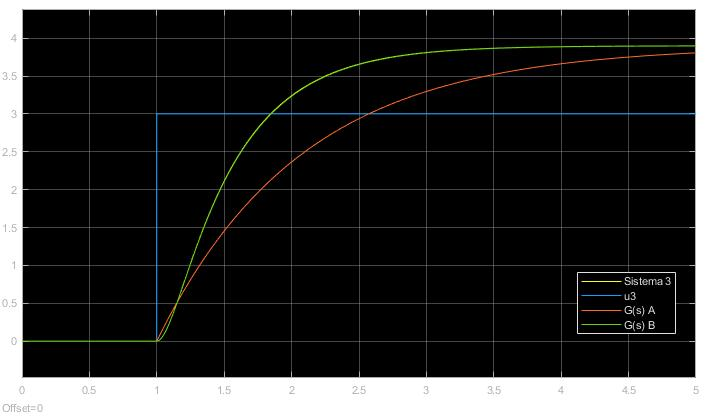
\includegraphics{Imagens/Lab3/Resolução/prob3BB.jpg}

Percebe-se que, considerando o modelo como uma Função de Transferência de segundo grau obtida através de \(F(s)\) é possível encontrar a curva exata correspondente ao Sistema 3.

\hypertarget{rastreamento-de-referuxeancias-e-rejeiuxe7uxe3o-de-perturbauxe7uxf5es---erro-em-regime-permanente}{%
\chapter{Rastreamento de Referências e Rejeição de Perturbações - Erro em Regime Permanente}\label{rastreamento-de-referuxeancias-e-rejeiuxe7uxe3o-de-perturbauxe7uxf5es---erro-em-regime-permanente}}

\hypertarget{apresentauxe7uxe3o-do-laboratuxf3rio-2}{%
\section{Apresentação do Laboratório}\label{apresentauxe7uxe3o-do-laboratuxf3rio-2}}

\hypertarget{objetivos}{%
\subsection{Objetivos}\label{objetivos}}

Nesta experiência analisaremos o erro em regime permanente de sistemas em malha-fechada para o rastreamento de referências e a rejeição de perturbações. Consideraremos referências e perturbações do tipo degrau, rampa e parábola. Comprovaremos os resultados teóricos através de simulações no Simulink/Matlab.

\hypertarget{tipos-de-sistemas}{%
\subsection{Tipos de Sistemas}\label{tipos-de-sistemas}}

Considere a Função de Transferência
\[
G(s) = \frac {N(s)}{D(s)}
\]
onde \(N(s)\) e \(D(s)\) são polinômios em \(s\) sem raízes em comum e com \(\text{grau}(N) \leq \text{grau}(D)\). Temos a seguinte classificação para \(G(s)\):

\begin{itemize}
\tightlist
\item
  Tipo 0: \(G(s)\) não possui pólos em \(s=0\). Denominamos \(K_p = G(0)\) de \emph{constante de posição}. Note que \(K_p = \lim\limits_{s \to 0} G(s)\).
\item
  Tipo 1: \(G(s)\) tem um (e apenas um) pólo em \(s=0\). Podemos então escrever \[G(s) = \frac {1}{s}G_0(s),\] onde \(G_0(s) = \frac {N(s)}{D_0(s)}\) não possui pólos em \(s=0\). Chamamos \(K_v= G_0(0) \neq 0\) de \emph{constante de velocidade}. Note que \(K_v = \lim\limits_{s \to 0} sG(s)\).
\item
  Tipo 2: \(G(s)\) tem dois (e apenas dois) pólos em \(s=0\). Podemos escrever \[G(s) = \frac {1}{s^2}G_0(s),\] onde \(G_0(s) = \frac {N(s)}{D_0(s)}\) não possui pólos em \(s=0\). Denominamos \(K_a = G_0(0) \neq 0\) de \emph{constante de aceleração}. Note que \(K_a =\lim\limits_{s \to 0} s^2G(s)\).
\end{itemize}

\hypertarget{erro-em-regime-permanente}{%
\subsection{Erro em regime permanente}\label{erro-em-regime-permanente}}

Considere o sistema em malha-fechada com realimentação unitária mostrado na Figura @ref\{fig:fig41\}, onde:
\[
\begin{cases}
  y(t) & \quad \text{: saída}\\
  r(t) & \quad \text{: referência}\\
  e(t) = r(t)-y(t) & \quad \text{: erro de rastreamento}\\
  w(t) &\quad \text{: perturbação externa que não é possível de ser medida}
\end{cases}
\]

\begin{figure}
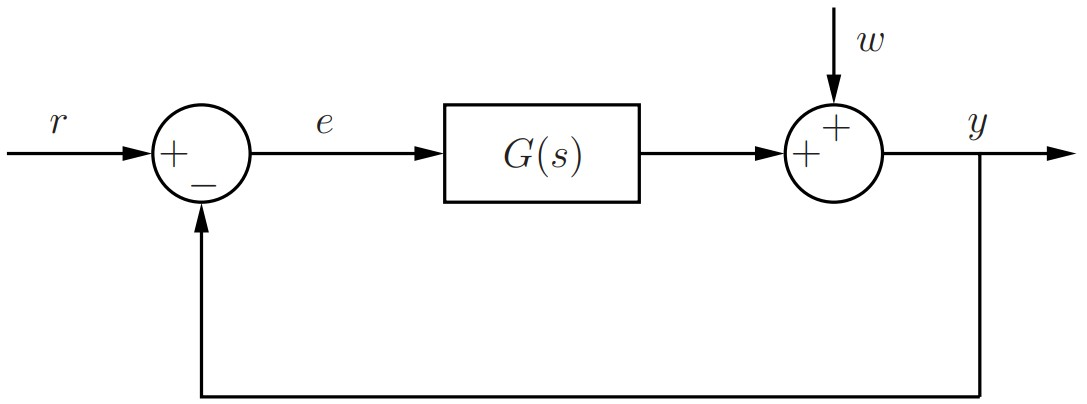
\includegraphics[width=0.8\linewidth]{Imagens/Lab4/Apresentação/fig1} \caption{Sistema em malha-fechada com perturbação na saída.}\label{fig:fig41}
\end{figure}

Desejamos analisar o erro em regime permanente (\(t \to \infty\)) quando existem perturbações externas. Temos que

\[
E(s) = R(s) - Y(s) = R(s) - [G(s)E(s) + W(s)]\\
\implies E(s) = \frac {1}{1 + G(s)}R(s) - \frac {1}{1+G(s)}W(s) \\
\implies E(s) = \underbrace{\frac {D(s)}{D(s) + N(s)}R(s)}_{E_R(s)} - \underbrace{\frac {D(s)}{D(s) + N(s)}W(s)}_{Y_W(s)}
\]

Note que \(E = E_R\) quando \(W= 0\) e que \(Y = Y_W\) quando \(R=0\). Podemos então analisar \(E\) através de \(E_R\) e \(Y_R\). O erro em regime permanente é dado por

\begin{align}
e(\infty) = \lim\limits_{t \to \infty}{e(t)} = e_r(\infty) - y_w(\infty), \label{eq:eq41}
\end{align}

desde que os limites \(e_r(\infty) = \lim\limits_{t\to \infty}{e_r(t)}\) e \(y_w(\infty) = \lim\limits_{t \to \infty}{y_w(t)}\) existam. Dizemos que há \emph{rastreamento de referência} quando \(e_r(\infty) = 0\). De maneira semelhante, dizemos que há \emph{rejeição de perturbação} quando \(y_w(\infty) = 0\). Portanto, quando há rastreamento de referência e rejeição de perturbação teremos que \(e(\infty) = 0\).

Iremos agora analisar \(e_r(\infty)\) e \(y_w(\infty)\) através de \(E_R(s)\) e \(Y_W(s)\), respectivamente, considerando que a referência \(r\) e a perturbação externa \(w\) são do tipo degrau, rampa ou parábola. Relembramos que:

\begin{enumerate}
\def\labelenumi{\arabic{enumi}.}
\tightlist
\item
  Degrau: \(x(t) = A \iff X(s) = \frac {A}{s}\)
\item
  Rampa: \(x(t) = Bt \iff X(s) = \frac {B}{s^2}\)
\item
  Parábola: \(x(t) = Ct^2 \iff X(s) = \frac {2C}{s^3}\)
\end{enumerate}

Suponha que \(D(s) + N(s) = 0\) possui todas as raízes no SPE (Semi-Plano Esquerdo do plano \(s\)) e que \(D(s)R(s)\) e \(D(s)W(s)\) possuem no máximo um pólo em \(s=0\). Isto garante que \(e_r(\infty)\) e \(y_w(\infty)\) existem e, assim, o Teorema do Valor Final pode ser aplicado. Ressaltamos que as raízes de \(D(s) + N(s) = 0\) nada mais são do que os pólos da Função de Transferência de malha-fechada quando não há perturbação (\(w=0\))
\[
F(s) = \frac {Y(s)}{R(s)} = \frac{G(s)}{1+G(s)} = \frac {N(s)}{D(s)+N(s)}, \quad \text{(para } w=0 \text{).} 
\]

Desse modo, estamos assumindo que \(F(s)\) é estável para \(w=0\). Com base no Teorema do Valor Final, podemos construir a tabela \ref{tab:tab1} e a tabela \ref{tab:tab2} mostradas abaixo. Note que os valores de \(e_r(\infty)\) e de \(y_w(\infty)\) (regime permanente) dependem apenas da constante de posição \(K_p\), da constante de velocidade \(K_v\) e da cosntante de aceleração \(K_a\). Tl nomenclatura tem origem em sistemas mecânicos de controle. Por exemplo, para um sistema Tipo 0 e \(r(t)=A\) (degrau) temos que (Teorema do Valor Final)
\[
e_r(\infty) = \lim\limits_{s \to 0}{sE_R(s)}=\lim\limits_{s\to0}{\frac{D(s)}{D(s)+N(s)}\frac{A}{s}} = \lim\limits_{s\to0}{\frac{AD(s)}{D(s)+N(s)}} \\
= \frac{AD(0)}{D(0) + N(0)} = \frac{A}{1+N(0)/D(0)} = \frac{A}{1+G(0)} = \frac {A}{1+K_p}.
\]
pois como \(D(0) + N(0) \neq 0\) (\(F(s)\) é estável) e \(D(0) \neq 0\) (\(G(0)\) é de Tipo 0) não há divisão por zero!

E, para um sistema Tipo 2 e \(r(t) = Bt\) (rampa), temos \(G(s) = \frac{N(s)}{D(s)} = \frac{N(s)}{s^2D_0(s)}\) e
\[
e_r(\infty) = \lim\limits_{s \to 0}{sE_r(s) = \lim\limits_{s \to 0}{s\frac{D(s)}{D(s)+N(s)}\frac{B}{s^2}}} = \lim\limits_{s \to 0}{s\frac{s^2D_0(s)}{D(s)+N(s)}\frac{B}{s^2}}\\
=\lim\limits_{s \to 0}{\frac{sBD_0(s)}{D(s)+N(s)}}=\frac{0BD(0)}{N(0)+D(0)}=0,
\]
pois \(D(0) + N(0) \neq 0\) (\(F(s)\) é estável) e não há divisão por zero!

Observamos que a tabela \ref{tab:tab1} e a tabela \ref{tab:tab2} são válidas apenas para sistemas com realimentação unitária com perturbação na saída (veja a Figura \ref{fig:fig41}) e tais que a Função de Transferência em malha-fechada é estável para \(w=0\).

\begin{table}

\caption{\label{tab:tab1}Valores de $e_r(\infty)$ ($w=0$)}
\centering
\begin{tabular}[t]{llll}
\toprule
Sistema $G(s)$ / Referência & $r(t)=A$ & $r(t) = Bt$ & $r(t) = Ct^2$\\
\midrule
Tipo 0 & $\frac{A}{1 + K_p}$ & $\infty$ & $\infty$\\
Tipo 1 & 0 & $\frac{B}{K_v}$ & $\infty$\\
Tipo 2 & 0 & 0 & $\frac{2C}{K_a}$\\
\bottomrule
\end{tabular}
\end{table}

\begin{table}

\caption{\label{tab:tab2}Valores de $y_r(\infty)$ ($r=0$ e $w$ na saída de $G(s)$)}
\centering
\begin{tabular}[t]{llll}
\toprule
Sistema $G(s)$ / Perturbação & $w(t)=A$ & $w(t) = Bt$ & $w(t) = Ct^2$\\
\midrule
Tipo 0 & $\frac{A}{1 + K_p}$ & $\infty$ & $\infty$\\
Tipo 1 & 0 & $\frac{B}{K_v}$ & $\infty$\\
Tipo 2 & 0 & 0 & $\frac{2C}{K_a}$\\
\bottomrule
\end{tabular}
\end{table}

Agora, considere o sistema mostrado na Figura \ref{fig:fig42} e assuma que \(G_2(s)\) não possui \emph{zeros} em \(s=0\). Para tal sistema, a Tabela \ref{tab:tab1} continua válida para \(G(s) = G_1(s)G_2(s)\). No entanto, a Tabela \ref{tab:tab2} deve ser substituída pela Tabela \ref{tab:tab3}. Ressaltamos que os valores \(\neq 0\) na Tabela \ref{tab:tab3} podem ser calculados analiticamente a partir de \(G_1(s) \text{ e } G_2(s)\). Entretanto, isso não é o objeto de estudo desta experiência.

\begin{figure}
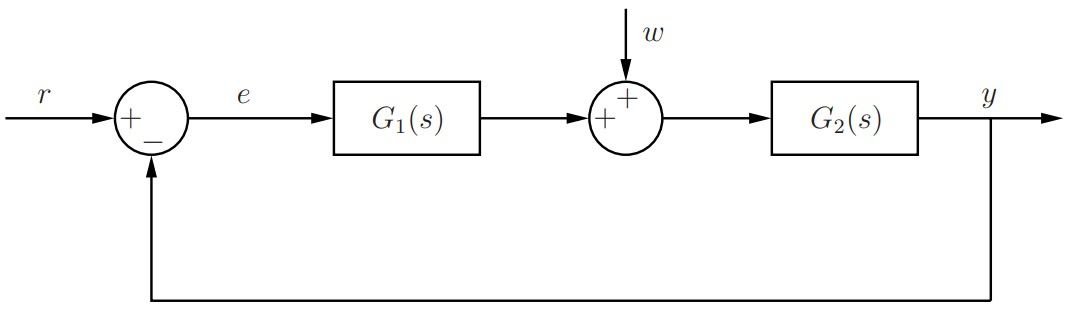
\includegraphics[width=0.8\linewidth]{Imagens/Lab4/Apresentação/fig2} \caption{Sistema em malha-fechada com perturbação na entrada de $G_s(s)$ e $G_2(s)$ não possui *zeros* em $s=0$.}\label{fig:fig42}
\end{figure}

\begin{table}

\caption{\label{tab:tab3}Valores de $y_r(\infty)$ ($r=0$ e $w$ na saída de $G_2(s)$)}
\centering
\begin{tabular}[t]{llll}
\toprule
Sistema $G(s)$ / Perturbação & $w(t)=A$ & $w(t) = Bt$ & $w(t) = Ct^2$\\
\midrule
Tipo 0 & $\neq 0$ & $\infty$ & $\infty$\\
Tipo 1 & 0 & $\neq 0$ & $\infty$\\
Tipo 2 & 0 & 0 & $\neq 0$\\
\bottomrule
\end{tabular}
\end{table}

\hypertarget{procedimentos-2}{%
\section{Procedimentos}\label{procedimentos-2}}

Em todos os itens abaixo consideramos o sistema em malha-fechada mostrado na Figura \ref{fig:fig43} onde \(C(s)\) é o controlador, \(G(s)\) é a planta (processo) e \(u(t)\) é o sinal de controle.

\begin{figure}
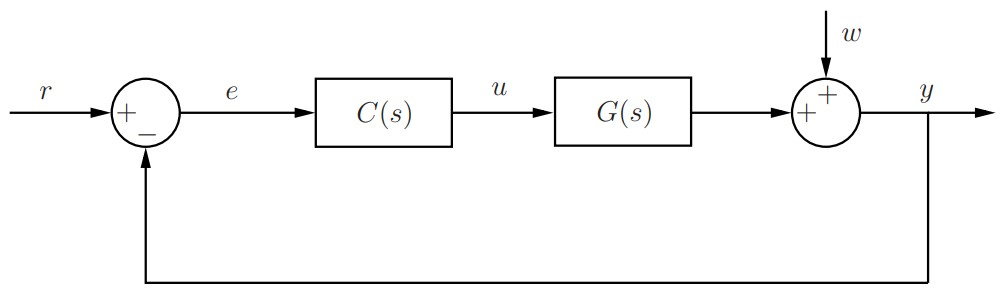
\includegraphics[width=0.8\linewidth]{Imagens/Lab4/Apresentação/fig3} \caption{Sistema em malha-fechada.}\label{fig:fig43}
\end{figure}

\hypertarget{problema-1-2}{%
\subsection*{Problema 1}\label{problema-1-2}}
\addcontentsline{toc}{subsection}{Problema 1}

Considere que

\[
G(s) = \frac {1}{0.5s+1}, \quad C(s) = K_c \quad \text{(proporcional)}, \quad w=0 \quad \text{(sem perturbação)}.
\]

\begin{enumerate}
\def\labelenumi{\alph{enumi}.}
\tightlist
\item
  Simule para \(r(t) = 1\) (degrau unitário) e \(K_c = 1\) Determine \(e(\infty) = e_r(\infty)\) por simulação e compare com a Tabela \ref{tab:tab1} (note que \(K_p = Kc\)). Repita para \(K_c = 10\) e \(K_c = 100\), analisando também o regime transitório de saída \(y(t)\).
\item
  Percebemos que \(e(\infty)\) diminui a medida que aumentamos o ganho \(K_c\) do controlador. Poderíamos então escolher \(K_c = \infty\) para que \(e(\infty) = 0\)? Justifique sua resposta (dica: observe o sinal de controle \(u(t)\)).
\item
  Com \(K_c = 1\) simule para \(r(t) = t\) (rampa) e \(r(t) = 0.5t^2\) (parábola). Determine o erro em regime permanente e verifique se os resultados estão de acordo com o esperado.
\end{enumerate}

\hypertarget{resoluuxe7uxe3o-10}{%
\subsubsection*{Resolução}\label{resoluuxe7uxe3o-10}}
\addcontentsline{toc}{subsubsection}{Resolução}

\hypertarget{parte-a-1}{%
\subsubsection*{Parte A}\label{parte-a-1}}
\addcontentsline{toc}{subsubsection}{Parte A}

Por meio da simulação foi encontrado o valor de \(e(\infty) = e_r(\infty) = 0.5\) conforme apresenta a Figura \ref{fig:fig41A1}.

\begin{figure}
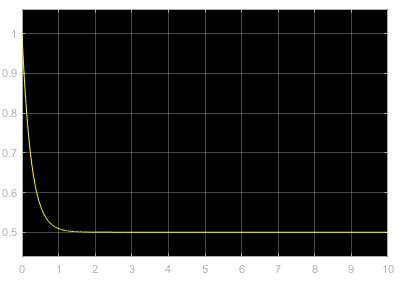
\includegraphics[width=0.8\linewidth]{Imagens/Lab4/Resolução/prob1A1} \caption{Valor de $e(r)$.}\label{fig:fig41A1}
\end{figure}

Utilizando a Tabela \ref{tab:tab1} temos que \(e_r(\infty)=\frac{A}{1 + K_p}\). Assim, tendo \(A = 1\) e \(K_c = 1\), temos que \(e_r(\infty) = \frac {1}{2} = 0.5\), o que está de acordo com o resultado encontrado na simulação. A figura \ref{fig:fig41A2} apresenta os valores de \(e(s) = e_r(s)\) e \(Y(s)\) para \(K_c = 10\) e \(K_c = 100\).

\begin{figure}
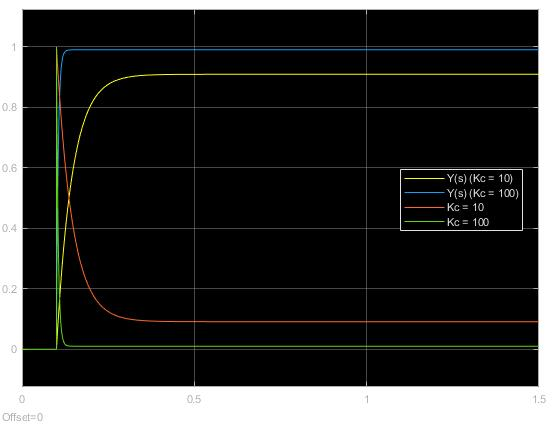
\includegraphics[width=0.8\linewidth]{Imagens/Lab4/Resolução/prob1A2} \caption{Valores para $K_c = 10$ e $K_c = 100$.}\label{fig:fig41A2}
\end{figure}

\hypertarget{parte-b-1}{%
\subsubsection*{Parte B}\label{parte-b-1}}
\addcontentsline{toc}{subsubsection}{Parte B}

Teoricamente, é possível encontrar um erro nulo \(e(\infty) = 0\) se utilizado um ganho infinito \(K_c = \infty\). Pois, de acordo com a Tabela \ref{tab:tab1}, temos que
\[
e(\infty) = \frac {A}{1+K_c} = \frac {A}{1+\infty} = 0.
\]

Entretanto, não existe um sistema prático que retorne um ganho infinito. O ideal seria considerar um sistema que seja de Tipo 1 ou 2 para que, ao aplicar uma entrada do tipo degrau ele retorne um erro nulo.

\hypertarget{parte-c}{%
\subsubsection*{Parte C}\label{parte-c}}
\addcontentsline{toc}{subsubsection}{Parte C}

A Figura \ref{fig:fig41C1} apresenta os valores de \(y(s)\) e \(e(s)\) para uma entrada \(r(t) = t\) (rampa).

\begin{figure}
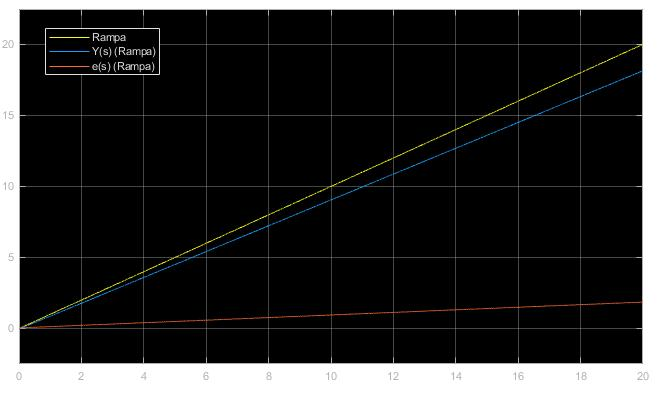
\includegraphics[width=0.8\linewidth]{Imagens/Lab4/Resolução/prob1C1} \caption{Valores para entrada do tipo rampa.}\label{fig:fig41C1}
\end{figure}

A Figura \ref{fig:fig41C2} apresenta os valores de \(y(s)\) e \(e(s)\) para uma entrada \(r(t) = 0.5t^2\) (parábola).

\begin{figure}
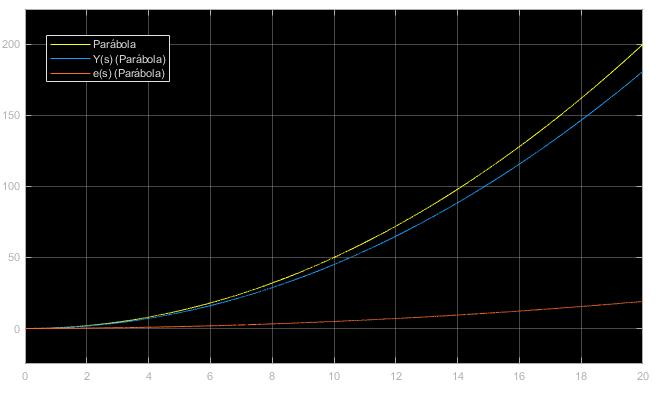
\includegraphics[width=0.8\linewidth]{Imagens/Lab4/Resolução/prob1C2} \caption{Valores para entrada do tipo parábola.}\label{fig:fig41C2}
\end{figure}

É possível perceber que, como o esperado, \(e(\infty)= e_r(\infty) = \infty\) para ambos os casos.

\hypertarget{problema-2-2}{%
\subsection*{Problema 2}\label{problema-2-2}}
\addcontentsline{toc}{subsection}{Problema 2}

Considere que
\[
G(s) = \frac {1}{0.5s+1}, \quad C(s) = \frac{K_c}{s} \text{ (integral)}, \quad w=0 \text{ (sem perturbação).}
\]

\begin{enumerate}
\def\labelenumi{\alph{enumi}.}
\tightlist
\item
  Simule para \(r(t) = 1\) (degrau unitário) e \(K_c = 1\). Determine \(e(\infty) = e_r(\infty)\) por simulação e compare com a Tabela \ref{tab:tab1}. Analise também o regime transitório da saída para \(y(t)\) (sobressinal, por exemplo). Repita para \(K_c = 10\). Observe o aumento no sobressinal.
\item
  Simule para \(K_c = 2\) e \(r(t) = t\) (rampa). Determine \(e(\infty)\) por simulação e compare com a Tabela \ref{tab:tab1} (note que \(K_v = K_c\)). Encontre analiticamente \(K_c\) de modo que o erro à rampa \(r(t) = t\) em regime permanente seja igual a 0.1. Agora verifique se as simulações estão de acordo com o valor calculado de \(K_c\).
\item
  Simule para \(K_c = 2\) e \(r(t) = 0.5t^2\) (parábola). Determine o erro em regime permanente por simulação e analise os resultados.
\item
  Agora suponha que
  \[
  G(s) = \frac {-s+2}{0.5s+1}, \quad C(s)= \frac{2}{s}, \quad r(t) = 1 \text{ (degrau).}
  \]
  Determine \(e(\infty)\) por simulação. Note que o erro não converge para zero. O resultado está de acordo com o esperado? Relembre que a Tabela \ref{tab:tab1} e a Tabela \ref{tab:tab2} são validas apenas quando o sistema em malha-fechada para \(w=0\) é estável (os pólos estão no SPE).
\end{enumerate}

\hypertarget{resuluuxe7uxe3o}{%
\subsubsection*{Resulução}\label{resuluuxe7uxe3o}}
\addcontentsline{toc}{subsubsection}{Resulução}

\hypertarget{parte-a-2}{%
\paragraph*{Parte A}\label{parte-a-2}}
\addcontentsline{toc}{paragraph}{Parte A}

Aplicando um controle \(C(s) = \frac {K_c}{s}\) em série a uma função \(G(s) = \frac {1}{0.5s+1}\) temos como resultado a Função de Transferência\\
\[
G_t(s) = C(s)G(s) = \frac {K_c}{s} \frac{1}{0.5s+1} = \frac {K_c}{s(0.5s+1)},
\]
que não possui zeros e possui pólos em \(s = 0\) e \(s = 2\). Deste modo, o sistema se caracteriza como um sistema do Tipo 1. Simulando o sistema temos como resultado a Figura \ref{fig:fig42A1}.

\begin{figure}
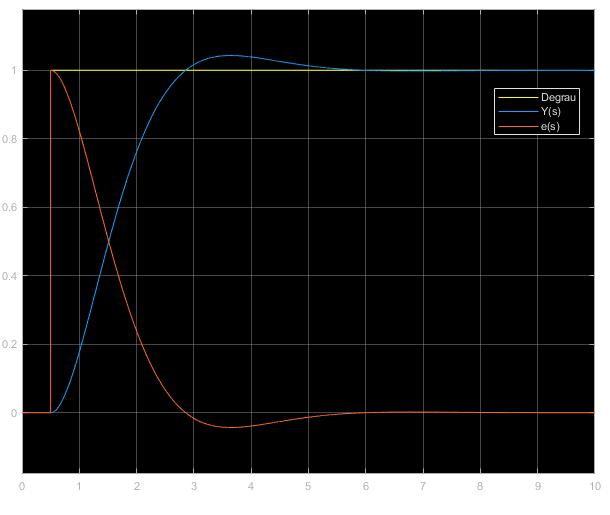
\includegraphics[width=0.8\linewidth]{Imagens/Lab4/Resolução/prob2A1} \caption{Valores para $K_c = 1$.}\label{fig:fig42A1}
\end{figure}

Simulando para \(K_c = 10\), temos o resultado abaixo.

\begin{figure}
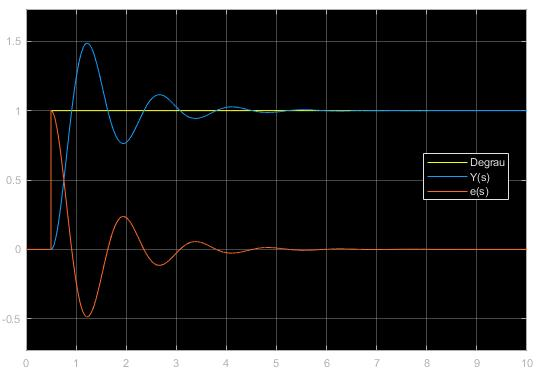
\includegraphics[width=0.8\linewidth]{Imagens/Lab4/Resolução/prob2A2} \caption{Valores para $K_c = 10$.}\label{fig:fig42A2}
\end{figure}

\hypertarget{parte-b-2}{%
\paragraph*{Parte B}\label{parte-b-2}}
\addcontentsline{toc}{paragraph}{Parte B}

Simulando o sistema para um \(K_c = 2\) e uma entrada tipo rampa, temos que o sistema tem \(e(\infty) = 0.5\), o que está de acordo com a Tabela \ref{tab:tab1}. O resultado da simulação está apresentado abaixo.

\begin{figure}
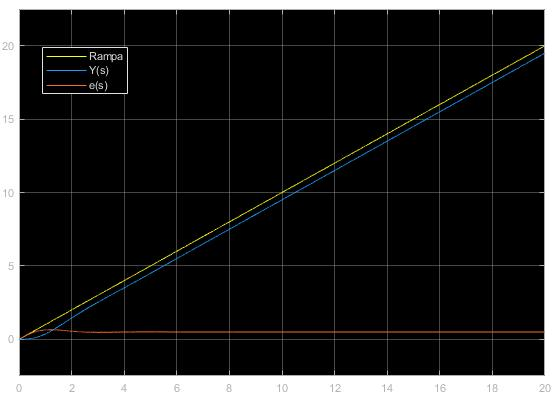
\includegraphics[width=0.8\linewidth]{Imagens/Lab4/Resolução/prob2B1} \caption{Valores para $K_c = 2$ e entrada do tipo rampa.}\label{fig:fig42B1}
\end{figure}

Analiticamente, é possível calcular o valor de \(K_v\) para que \(e(\infty) = 0.1\).

\[
0.1 = \frac {1}{K_v} \implies K_v = 10
\]

Simulando o sistema o valor foi comprovado.

\begin{figure}
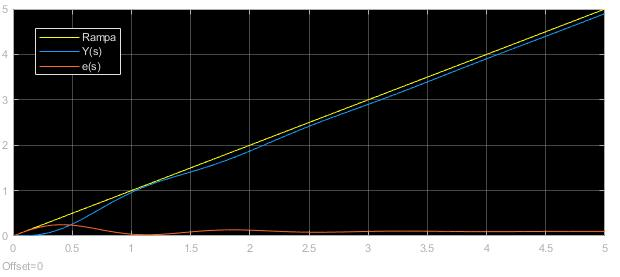
\includegraphics[width=0.8\linewidth]{Imagens/Lab4/Resolução/prob2B2} \caption{Valores para $K_c = 10$ e entrada do tipo rampa.}\label{fig:fig42B2}
\end{figure}

\hypertarget{parte-c-1}{%
\paragraph*{Parte C}\label{parte-c-1}}
\addcontentsline{toc}{paragraph}{Parte C}

Simulando o sistema para \(K_c = 2\) e uma entrada do tipo parábola, temos \(e(\infty) = \infty\), o que está de acordo com a Tabela \ref{tab:tab1}.

\begin{figure}
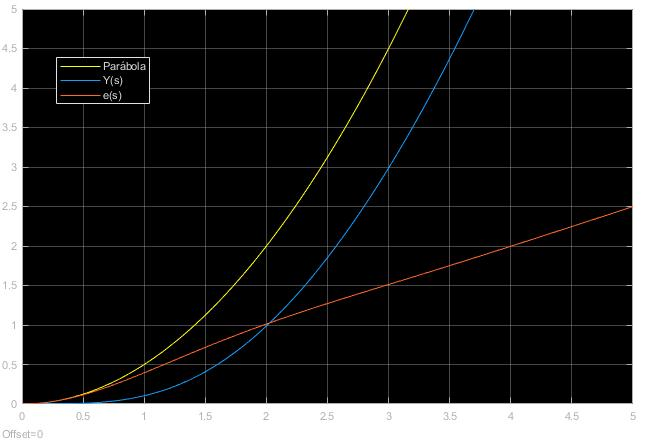
\includegraphics[width=0.8\linewidth]{Imagens/Lab4/Resolução/prob2C1} \caption{Valores para $K_c = 2$ e entrada do tipo parábola.}\label{fig:fig42C1}
\end{figure}

\hypertarget{parte-d}{%
\paragraph*{Parte D}\label{parte-d}}
\addcontentsline{toc}{paragraph}{Parte D}

Simulando a Função de Transferência \(G(s) = \frac {-s+2}{0.5s +1}\), controle \(C(s) = \frac {2}{s}\) e entrada do tipo degrau temos o resultado apresentado na Figura \ref{fig:fig42D1}.

\begin{figure}
\includegraphics[width=0.8\linewidth]{Imagens/Lab4/Resolução/prob2D1} \caption{Valores de $e(s)$ e $y(s)$.}\label{fig:fig42D1}
\end{figure}

Diferentemente do esperado (que o \(e(\infty) = 0\)) uma vez que segundo a Tabela \ref{tab:tab1} para sistemas do Tipo 1 para entrada igual degrau o erro esperado é nulo, o erro não converge. Na realidade, é possível notar que o sistema não se comportou de forma estável.

\hypertarget{problema-3-2}{%
\subsection*{Problema 3}\label{problema-3-2}}
\addcontentsline{toc}{subsection}{Problema 3}

Considere que
\[
G(s) = \frac {1}{0.5s +1}, \quad C(s) = \frac {2}{s} \text{ (integral)}.
\]

\begin{enumerate}
\def\labelenumi{\alph{enumi}.}
\tightlist
\item
  Determine \(y(\infty) = y(\infty)\) por simulação para \(w =1\) (degrau unitário) e \(r=0\). Compare com a Tabela \ref{tab:tab2}.
\item
  considere que \(r(t) = 5\) (degrau em \(t=0\)) e aplique uma perturbação \(w=1\) (degrau) no instante \(t=9\). Determine \(e(\infty)\) e analise os resultados (talvez seja necessário aumentar o tempo de simulação).
\item
  Considere que \(r(t) = 2t\) (rampa) e \(w=0\). Determine \(e(\infty) = e_r(\infty)\) por simulação e compare com a Tabela \ref{tab:tab1}.
\item
  Considere que \(r(t) = 0\) e \(w=t\) (rampa). Determine \(y(\infty) = y_w(\infty)\) por simulação e compare com a Tabela \ref{tab:tab2}.
\item
  Considere que \(r(t) = 2t\) (rampa) e \(w=t\) (rampa). Determine \(e(\infty)\) por simulação e verifique que tal valor é a diferença dos valores obtidos nas letras c e d.~Tal resultado era esperado? Justifique (relembre \eqref{eq:eq41}).
\end{enumerate}

\hypertarget{resoluuxe7uxe3o-11}{%
\subsubsection*{Resolução}\label{resoluuxe7uxe3o-11}}
\addcontentsline{toc}{subsubsection}{Resolução}

Working on it :)

\hypertarget{projeto-de-controladores-por-muxe9todos-alguxe9bricos}{%
\chapter{Projeto de Controladores por Métodos Algébricos}\label{projeto-de-controladores-por-muxe9todos-alguxe9bricos}}

Working on it :)

\hypertarget{linearizauxe7uxe3o-de-sistemas-nuxe3o-lineares}{%
\chapter{Linearização de Sistemas Não-Lineares}\label{linearizauxe7uxe3o-de-sistemas-nuxe3o-lineares}}

Working on it :)

\hypertarget{controle-de-sistemas-nuxe3o-lineares}{%
\chapter{Controle de Sistemas Não-Lineares}\label{controle-de-sistemas-nuxe3o-lineares}}

Working on it :)

\hypertarget{anuxe1lise-pelo-lugar-das-rauxedzes}{%
\chapter{Análise pelo Lugar das Raízes}\label{anuxe1lise-pelo-lugar-das-rauxedzes}}

Working on it :)

\hypertarget{projeto-de-controladores-pelo-lugar-das-rauxedzes}{%
\chapter{Projeto de Controladores pelo Lugar das Raízes}\label{projeto-de-controladores-pelo-lugar-das-rauxedzes}}

Working on it :)

\hypertarget{projeto-do-controlador-atraso-de-fase}{%
\chapter{Projeto do controlador atraso de fase}\label{projeto-do-controlador-atraso-de-fase}}

Working on it :)

\hypertarget{anuxe1lise-pelos-diagramas-de-bode-e-nyquist}{%
\chapter{Análise pelos Diagramas de Bode e Nyquist}\label{anuxe1lise-pelos-diagramas-de-bode-e-nyquist}}

Working on it :)

\hypertarget{projeto-de-controladores-pelo-diagrama-de-bode}{%
\chapter{Projeto de Controladores pelo Diagrama de Bode}\label{projeto-de-controladores-pelo-diagrama-de-bode}}

Working on it :)

\hypertarget{digitalizauxe7uxe3o-de-controladores-analuxf3gicos}{%
\chapter{Digitalização de Controladores Analógicos}\label{digitalizauxe7uxe3o-de-controladores-analuxf3gicos}}

Working on it :)

  \bibliography{book.bib,packages.bib}

\end{document}
